\documentclass[11pt]{article}
\usepackage[margin=1in]{geometry}
\usepackage{amsmath,amssymb,bm,graphicx,booktabs,caption,subcaption}
\usepackage[table]{xcolor}\usepackage{hyperref}\hypersetup{colorlinks=true,linkcolor=blue!50!black}
\graphicspath{{figs/}}\captionsetup{font=small}
\title{\textbf{A recurrent vision transformer shows signatures of primate visual attention:\\
a full-figure reproduction with a learned-from-pixels multiplicative-gating variant}}
\author{Reproduction of Morgan, Albanna \& Herman with the conv-frontend, $d_{\mathrm{mem}}{=}128$ \emph{element-wise multiplicative-gating} JEPA variant}
\date{Model checkpoint iteration 6{,}599 (task: 4-stimulus \texttt{vda4}, $50\times50$)}
\begin{document}\maketitle
\begin{abstract}\noindent
We reproduce \emph{every} figure of Morgan, Albanna \& Herman---the behavioural psychometrics and
chronometrics, the intrinsic attention dynamics, the feedback-mechanism comparison, the full decoding
battery, the actor-logit geometry, the reinforcement-learning value/TD/entropy analyses, the
signal-detection ``stimulation'' experiments, and the supervised-vs-RL comparison---using a variant of
the recurrent vision transformer that differs from the original in three ways: (i) the VAE
pre-processor is replaced by a small squeeze-and-excitation \emph{convolutional} front-end trained
end-to-end from pixels; (ii) the recurrent memory is a compact $d_{\mathrm{mem}}{=}128$ spatial xLSTM;
and (iii) the memory$\to$vision feedback is realised as \emph{element-wise multiplicative gating}, in
which the recurrent memory produces an affine transform $X'{=}\gamma(H)\odot X+\beta(H)$ of the visual
tokens before self-attention. The variant is trained purely from sparse reward with an auxiliary
temporal self-distillation (JEPA) objective. Like the original it produces orderly sigmoidal
psychometric/chronometric functions and a clear cued$>$uncued cueing benefit; its recurrent
self-attention shows interpretable spatial dynamics that reactivate priorities before the change; change
information is decodable from the mnemonic percept and is amplified across memory slots by
self-attention; the actor logits form a competitive Declare/Wait axis graded by change magnitude; the
distributional critic exhibits a value jump at the change; and---most directly answering the
``stimulation'' analyses---graded attention biasing lowers the signal-detection \emph{criterion} at the
attended location and modulates \emph{sensitivity} according to whether attention is directed toward or
away from the true change. We also report where this variant \emph{diverges}: its behaviour and
attention are largely \emph{invariant to displayed cue validity}, and---unlike the cross-attention
variant---its \emph{hard} attention clamps are a weaker causal lever on behaviour (the graded biasing
used in the SDT analysis remains effective). All figures are reproduced with this variant's data.
\end{abstract}

\section{Introduction}
The original model shows that a recurrent vision transformer trained by reinforcement learning on a
cued orientation-change task recapitulates hallmark behavioural and attentional signatures of primate
spatial attention. Here we ask whether these signatures survive three simplifications that make the
model learn perception from pixels and shrink its memory: a convolutional front-end in place of the
VAE, an element-wise multiplicative-gating memory$\to$vision feedback, and a $d_{\mathrm{mem}}{=}128$ recurrent state. We
reproduce \emph{each} figure of the original---main and supplementary---with this variant and note the
points of agreement and the single point of divergence (cue validity).

\section{Task and model}
The task is identical to the original (Fig.~\ref{fig:task}): each 7-step trial presents a $50\times50$
image sequence---blank, a spatial cue at $S_1$ or $S_4$ ($t{=}1$), blank, then four Gabor patches from
$t{=}3$; on half of trials one patch's orientation steps by $\Delta$ at $t{=}5$. A coloured cue signals
value and a ring signals validity. Because our environment samples the non-cued change location
uniformly, the empirical change-location probability at the cued patch is somewhat higher than the
nominal validity (e.g.\ $46\%$ at the $25\%$ ring; Fig.~\ref{fig:task}B). The variant
(Fig.~\ref{fig:model}) parses each frame into four patches, encodes them with a shared SE-ResNet, and
feeds the tokens to a recurrent transformer whose four visual tokens are first affinely modulated by the
memory ($X'{=}\gamma(H)\odot X+\beta(H)$) and then attend to one another; a spatial xLSTM holds the
working memory read out to a distributional actor--critic and distilled by a JEPA head.

\begin{figure}[h]\centering
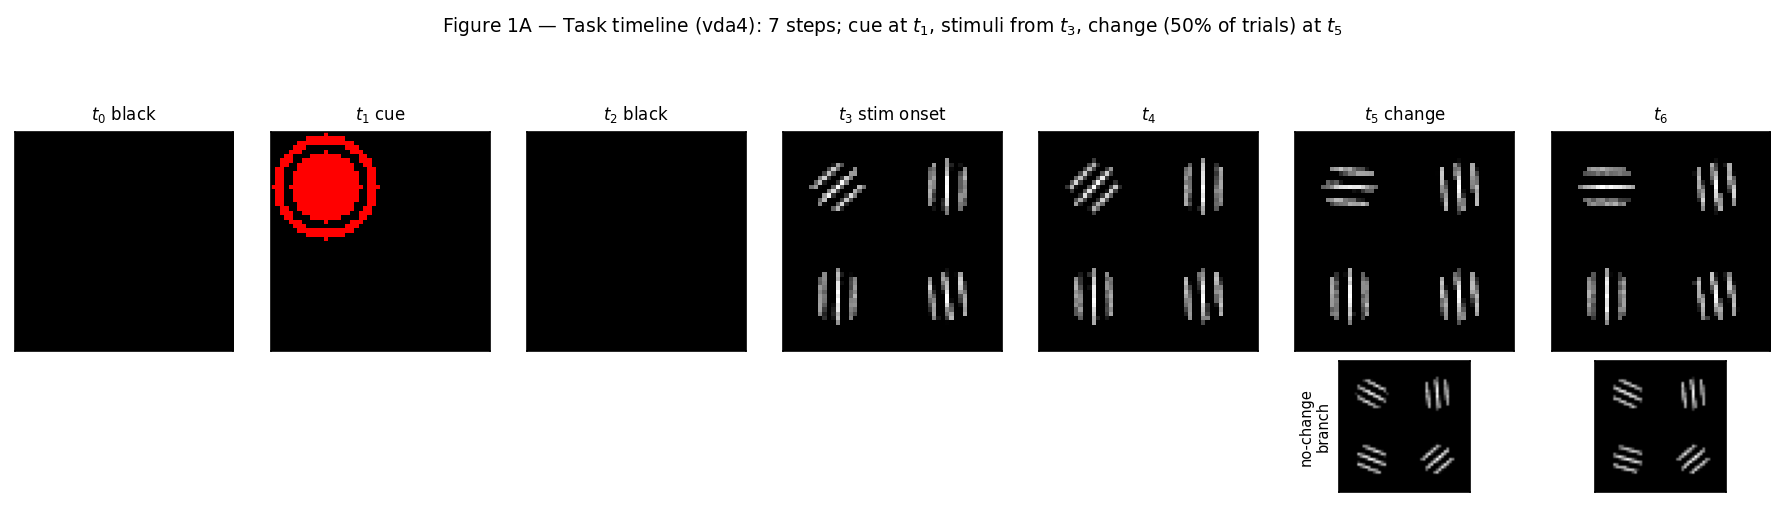
\includegraphics[width=\textwidth]{fig1A_task_timeline.png}\\[4pt]
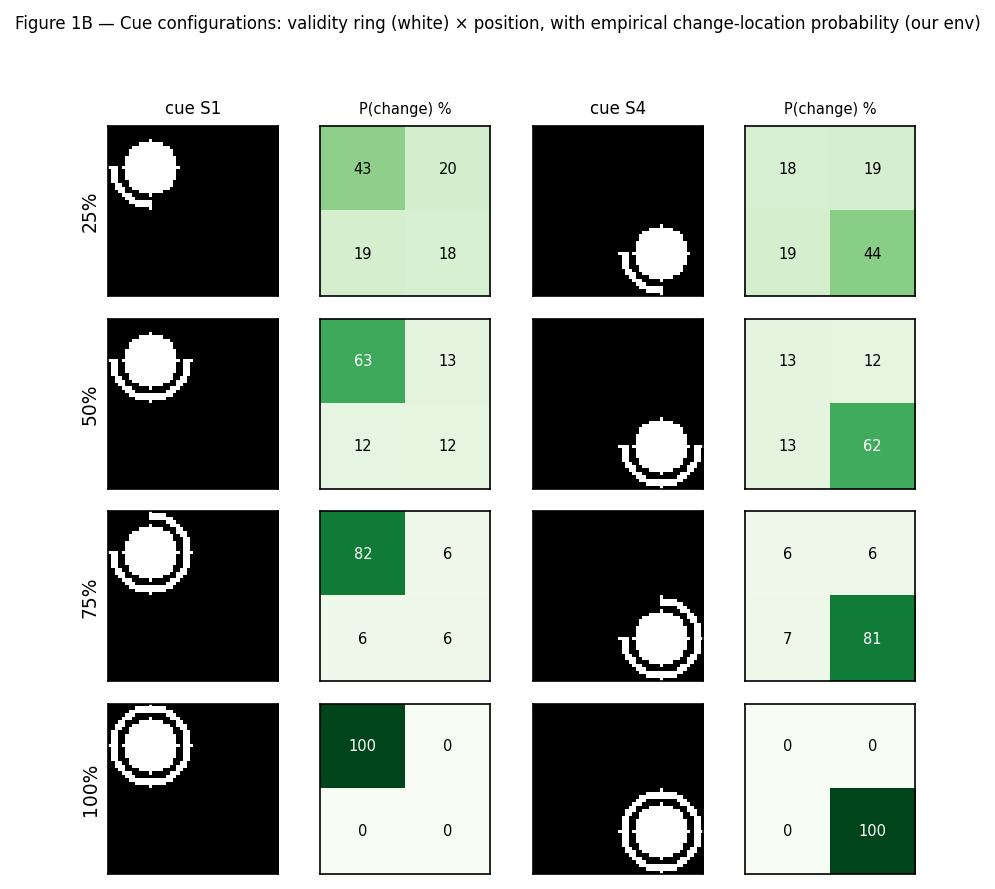
\includegraphics[width=0.6\textwidth]{fig1B_cue_configs.png}
\caption{\textbf{Fig 1 --- Task / environment.} Top: the 7-step trial timeline with the change /
no-change branch. Bottom: cue configurations (validity ring $\times$ position) with the empirical
change-location probability our environment produces.}\label{fig:task}\end{figure}

\begin{figure}[h]\centering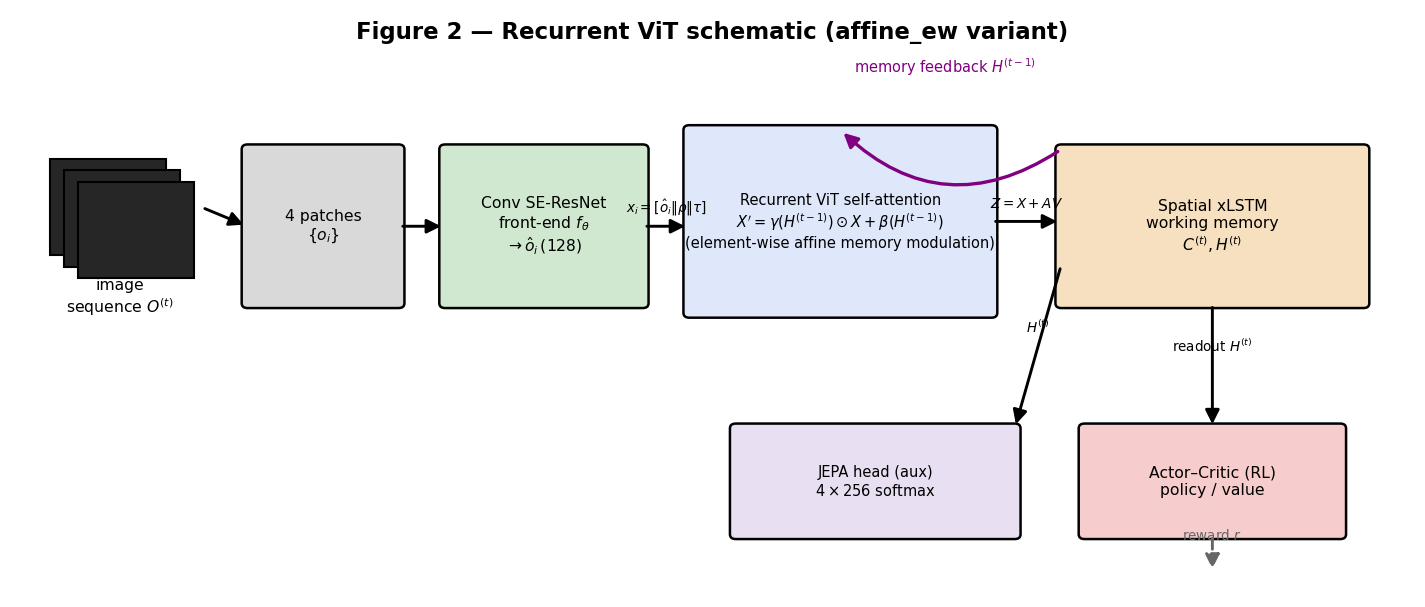
\includegraphics[width=\textwidth]{fig2_schematic_affine_ew.png}
\caption{\textbf{Fig 2 --- Model schematic (multiplicative-gating variant).} Image sequence $\to$ four
patches $\to$ conv SE-ResNet front-end $\to$ recurrent-ViT self-attention whose visual tokens are affinely
gated by the memory ($X'{=}\gamma(H)\odot X+\beta(H)$) $\to$ spatial xLSTM working memory $\to$ readout to
actor--critic (RL) and a JEPA head.}\label{fig:model}\end{figure}

\section{Behaviour: psychometrics and chronometrics}
The variant produces orderly sigmoidal psychometric and chronometric functions
(Fig.~\ref{fig:psy}) with the characteristic shapes of the original: response rate rises with $\Delta$,
floors near the false-alarm rate at $\Delta{=}0$, and saturates by $\sim\!30^\circ$; reaction time
decreases with $\Delta$. \emph{Divergence from the original:} the four validity conditions
($25/50/75/100\%$) are nearly superimposed, and the fitted logistic threshold (\emph{Position}) is flat
across validity ($12.5/12.8/13.1/12.3^\circ$). This variant therefore does \emph{not} reproduce the
original's validity-graded threshold shift---consistent with its perceiving the validity ring at the
cue frame but not retaining it. Fitted parameters are in Fig.~\ref{fig:psyp}.

\begin{figure}[h]\centering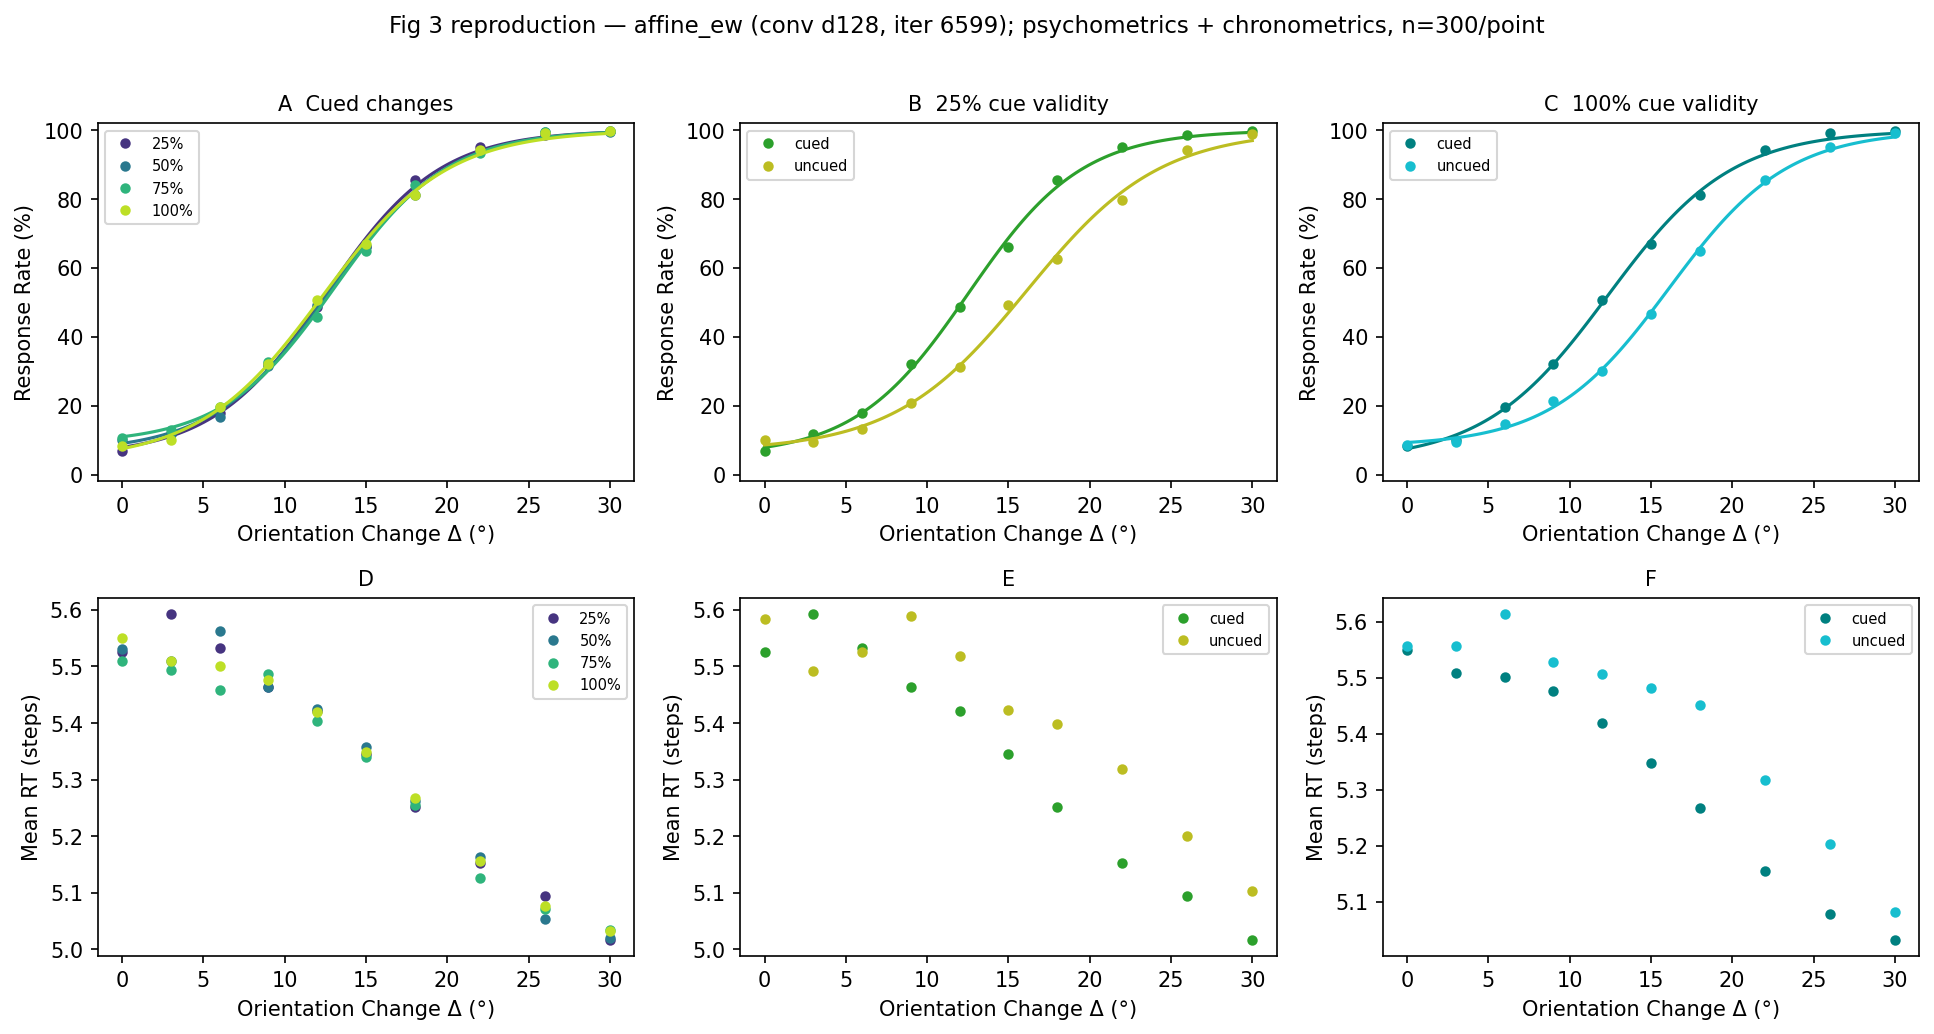
\includegraphics[width=\textwidth]{fig3_affine_ew.png}
\caption{\textbf{Fig 3 --- psychometrics and chronometrics.} A: response rate vs.\ $\Delta$ for cued
changes at four validities (superimposed for this variant). B, C: cued vs.\ uncued at $25\%$ and
$100\%$. D--F: mean reaction time. Points $n{=}300$; lines are 4-parameter logistic fits.}\label{fig:psy}\end{figure}
\begin{figure}[h]\centering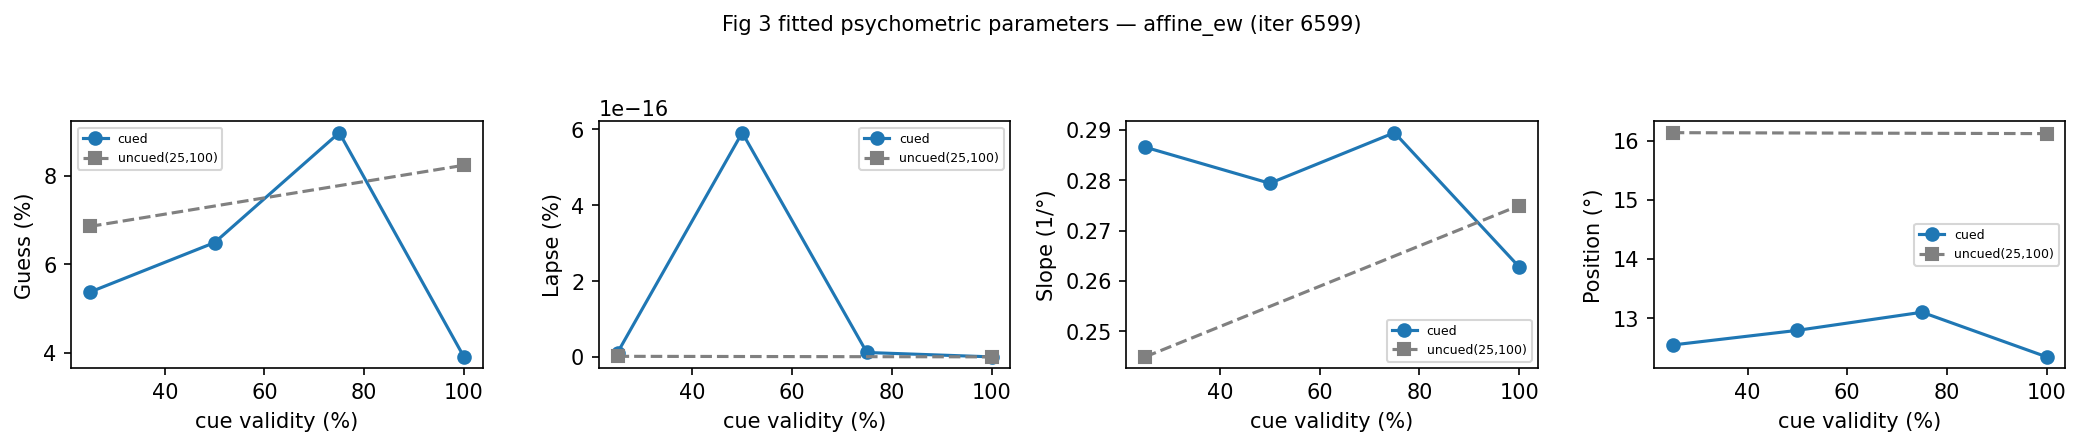
\includegraphics[width=0.95\textwidth]{fig3_affine_ew_params.png}
\caption{\textbf{Fitted psychometric parameters} (guess, lapse, slope, position) vs.\ cue validity, cued
and uncued.}\label{fig:psyp}\end{figure}

\section{Attention allocation dynamics}
Averaged recurrent self-attention (Fig.~\ref{fig:attn}) is flat at onset, becomes strongly biased
toward the cued location at the cue frame ($\alpha_1{\approx}0.74$ at $t{=}1$), and---because memory
sustains allocation without visual input---remains biased through the following blank. This anticipatory
maintenance of spatial priority in memory reproduces a core feature of the original. Panel B shows
$\alpha_1,\alpha_4$ across time; panel C shows $\alpha_1$ at the change frame vs.\ change magnitude at
the cued/uncued locations. Time-courses are again essentially \emph{invariant to displayed validity}.

\begin{figure}[h]\centering
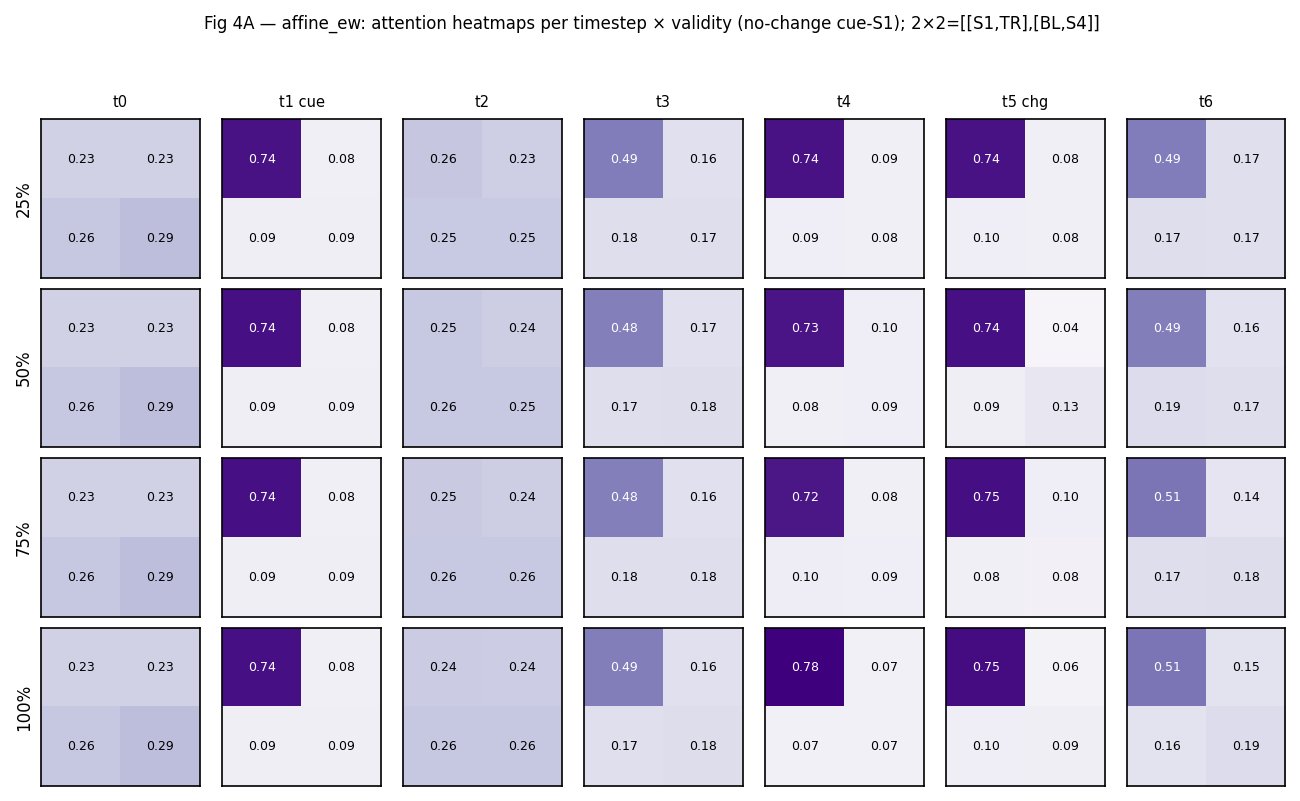
\includegraphics[width=\textwidth]{fig4A_affine_ew.png}\\[4pt]
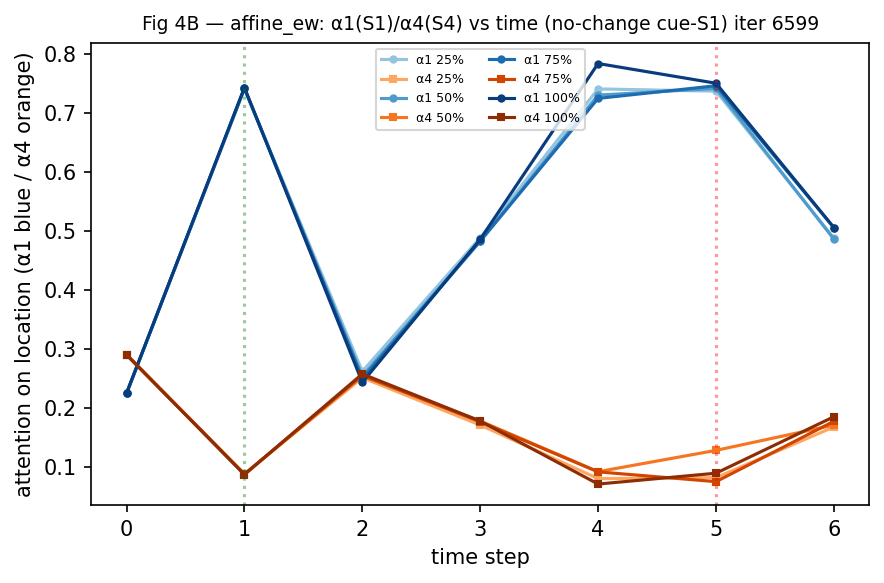
\includegraphics[width=0.47\textwidth]{fig4B_affine_ew.png}\hfill
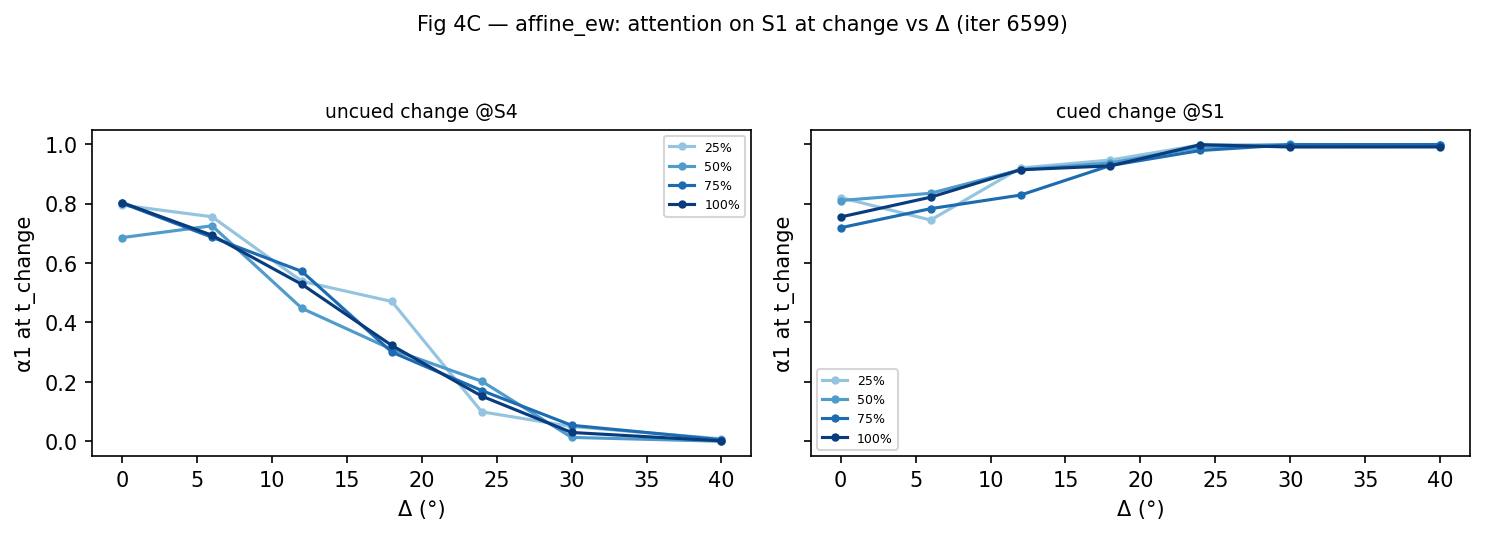
\includegraphics[width=0.47\textwidth]{fig4C_affine_ew.png}
\caption{\textbf{Fig 4 --- intrinsic attention dynamics.} Top: per-timestep attention heatmaps
($2\times2$) by validity on no-change cue-$S_1$ trials. Bottom left: $\alpha_1$/$\alpha_4$ vs.\ time.
Bottom right: $\alpha_1$ at the change frame vs.\ $\Delta$ at the uncued and cued locations.}\label{fig:attn}\end{figure}

\section{Feedback mechanism}
The original compares three memory$\to$vision feedback mechanisms (concatenation / additive /
multiplicative); our variant instantiates the \emph{multiplicative} mechanism, in which the memory
gates the visual tokens element-wise ($X'{=}\gamma(H)\odot X+\beta(H)$) before self-attention---the
mechanism the original selected as its focus. Fig.~\ref{fig:fb} shows this variant's feedback circuit
alongside the four behavioural panels of the original's feedback figures: cued response by validity (A),
the behavioural effect of enhancing/suppressing attention on the cued change (B), cued vs.\ uncued at
$100\%$ (C), and the deployment of attention at the change frame (D).

\begin{figure}[h]\centering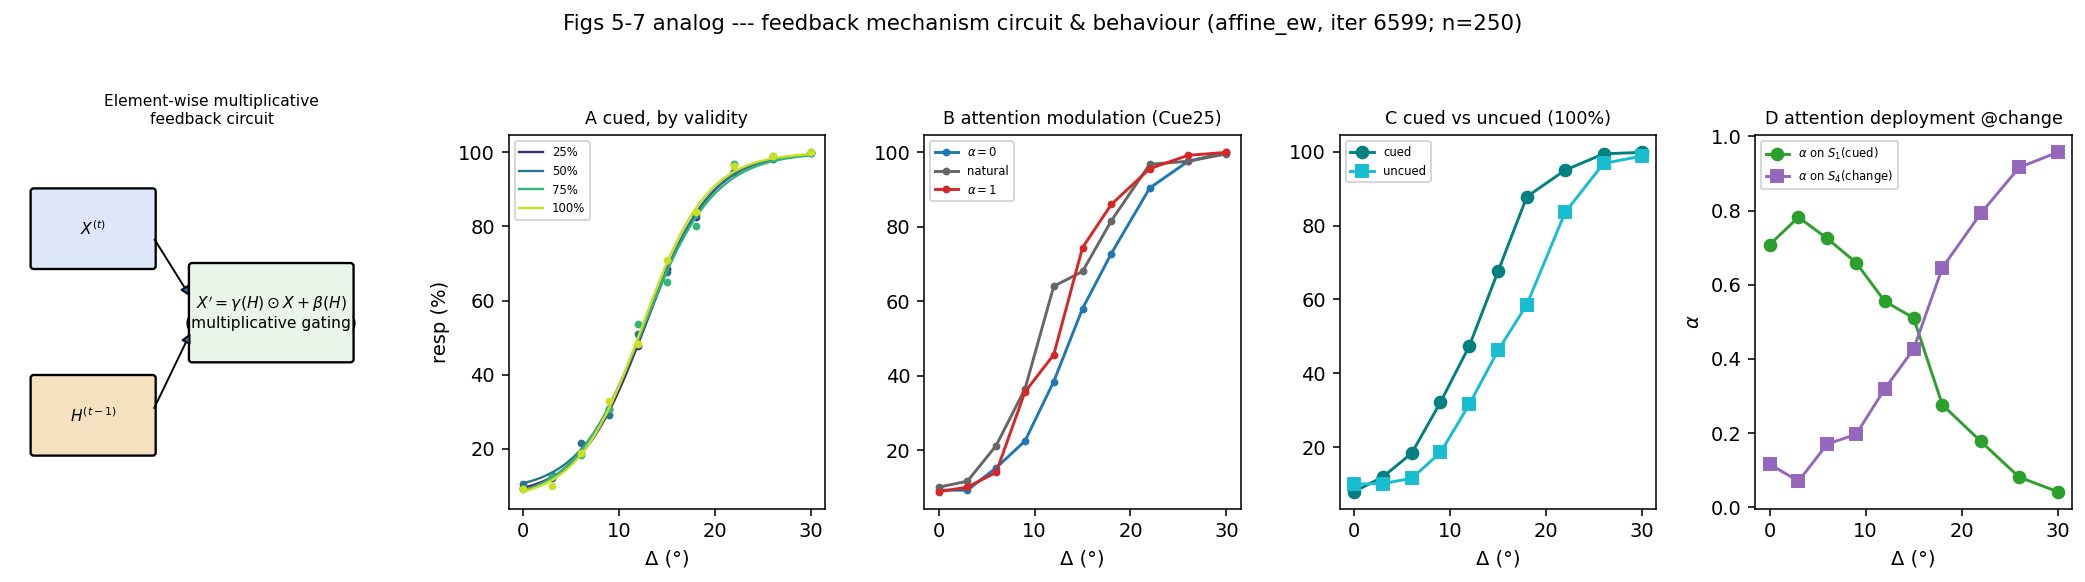
\includegraphics[width=\textwidth]{fig567_affine_ew.png}
\caption{\textbf{Figs 5--7 analog --- feedback mechanism circuit \& behaviour.} Left: the variant's
element-wise multiplicative-gating feedback circuit. A: cued response rate by validity. B: response under
enhanced/suppressed attention on the cued change. C: cued vs.\ uncued at $100\%$. D: attention deployed
on the cued ($S_1$) vs.\ change ($S_4$) location at the change frame vs.\ $\Delta$.}\label{fig:fb}\end{figure}

\section{Causal attention manipulations on behaviour}
We perturb the recurrent self-attention by \emph{hard}-clamping the attention allocated to a location at
the change frame (Fig.~\ref{fig:manip}). \emph{Divergence from the cross-attention variant:} for this
multiplicative-gating variant the hard clamps are a \emph{weak} causal lever on behaviour---directing
attention onto an \emph{uncued} change ($\alpha_4{=}1$) does not raise detection (at $\Delta{=}18^\circ$,
$0.65\to0.65$), and \emph{suppressing} the cued location ($\alpha_1{=}0$) slightly lowers it
($0.65\to0.61$); the ``dual effect'' is absent, and the parametric hard shift leaves the psychometric
threshold essentially flat (\emph{Position} $\approx\!12.2$--$13.4^\circ$ across $\alpha_1$;
Fig.~\ref{fig:manipp}). The attention here is real and interpretable but---because it enters
multiplicatively rather than as a competitive key/value---overriding it post-hoc has less behavioural
leverage than in the cross-attention variant. (The \emph{graded} biasing used for the SDT analysis,
Fig.~\ref{fig:sdt16}, nonetheless modulates the decision variable; see below.)

\begin{figure}[h]\centering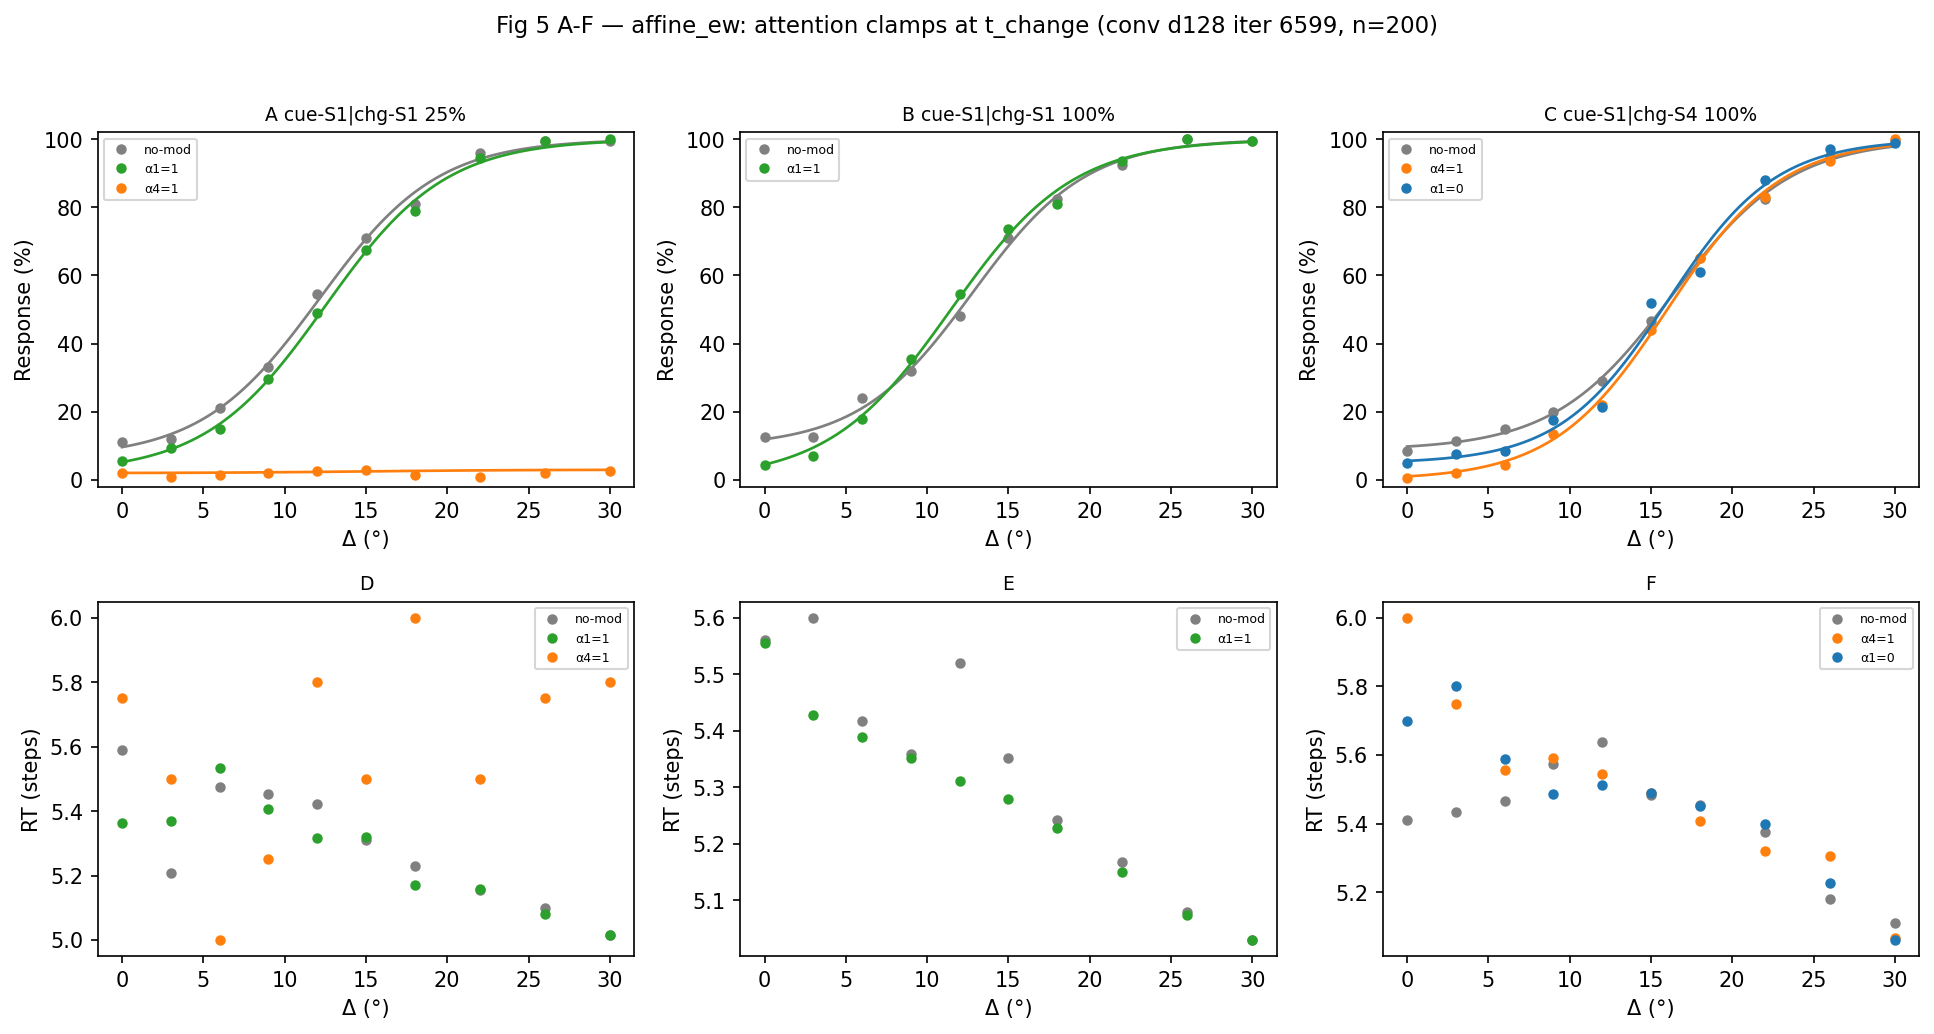
\includegraphics[width=\textwidth]{fig5AF_affine_ew.png}
\caption{\textbf{Attention clamps at $t_{\mathrm{change}}$.} Response rate (A--C) and reaction time
(D--F). For this variant the clamps produce little behavioural change (no dual effect).}\label{fig:manip}\end{figure}
\begin{figure}[h]\centering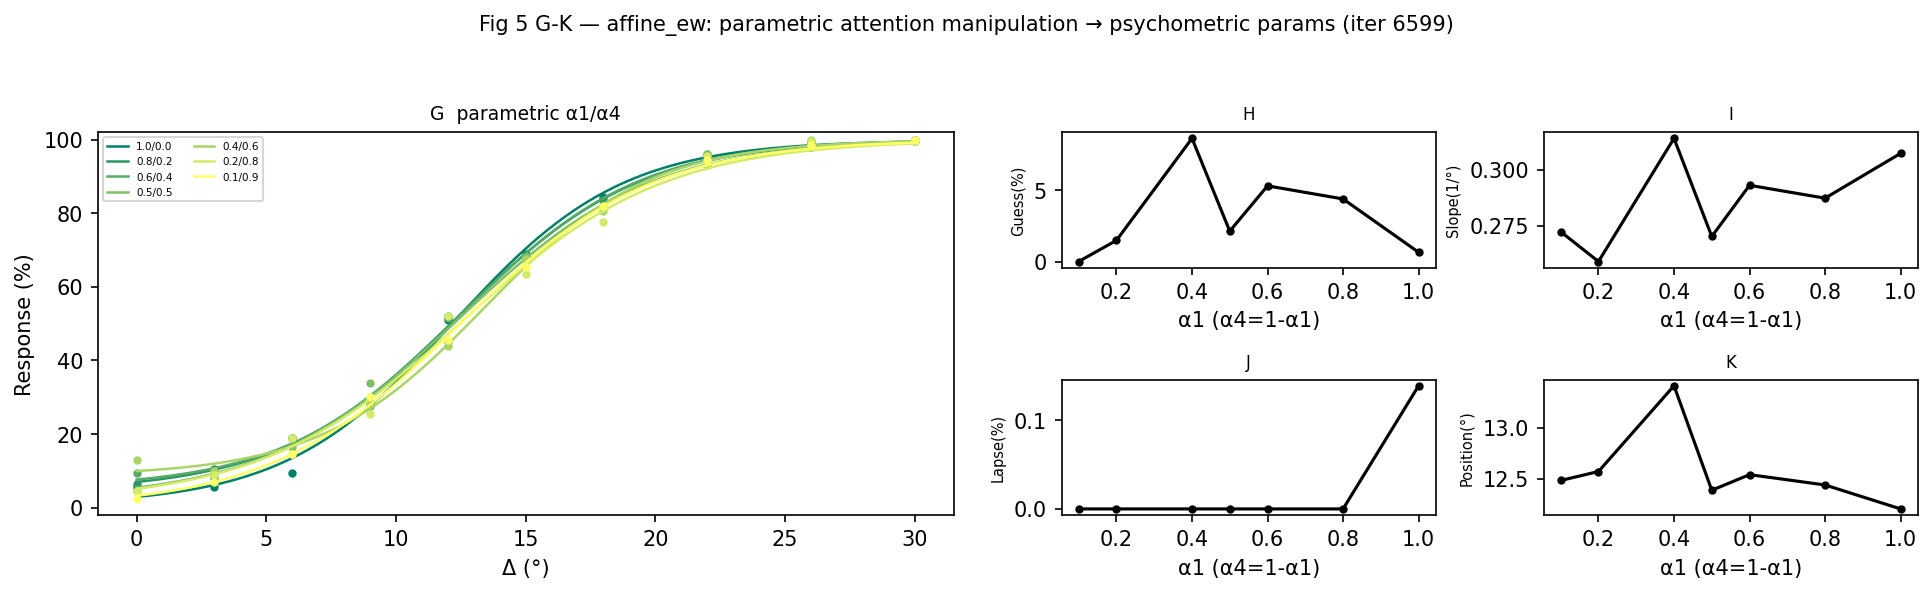
\includegraphics[width=\textwidth]{fig5GK_affine_ew.png}
\caption{\textbf{Parametric manipulation.} Shifting attention from uncued to cued leaves the psychometric
threshold nearly flat for this variant.}\label{fig:manipp}\end{figure}

\section{Decoding the mnemonic percept}
We train small feed-forward decoders (Linear--LayerNorm--ELU) on the recurrent states generated under
\emph{natural} (unmodulated) trials, then evaluate confusion matrices under attention modulation on
$S_1$. Change \emph{location} is decodable from the full mnemonic percept $H$
(Fig.~\ref{fig:dec8}), with decodability enhanced from $t{=}5$ to $t{=}6$ (temporal integration);
consistent with this variant's weaker attentional leverage, the modulation conditions
($\alpha_1{=}0/1$, spread) shift the confusion structure only modestly. From a \emph{single} patch $h_1$,
change \emph{occurrence} is decodable above chance (Fig.~\ref{fig:dec9}), indicating that self-attention
propagates the change signal across memory slots. The actor's first activation layer retains change
\emph{occurrence} but loses spatial specificity (Fig.~\ref{fig:dec10}), and graded inhibition of
$\alpha_1$ is examined in Fig.~\ref{fig:dec11}.

\begin{figure}[h]\centering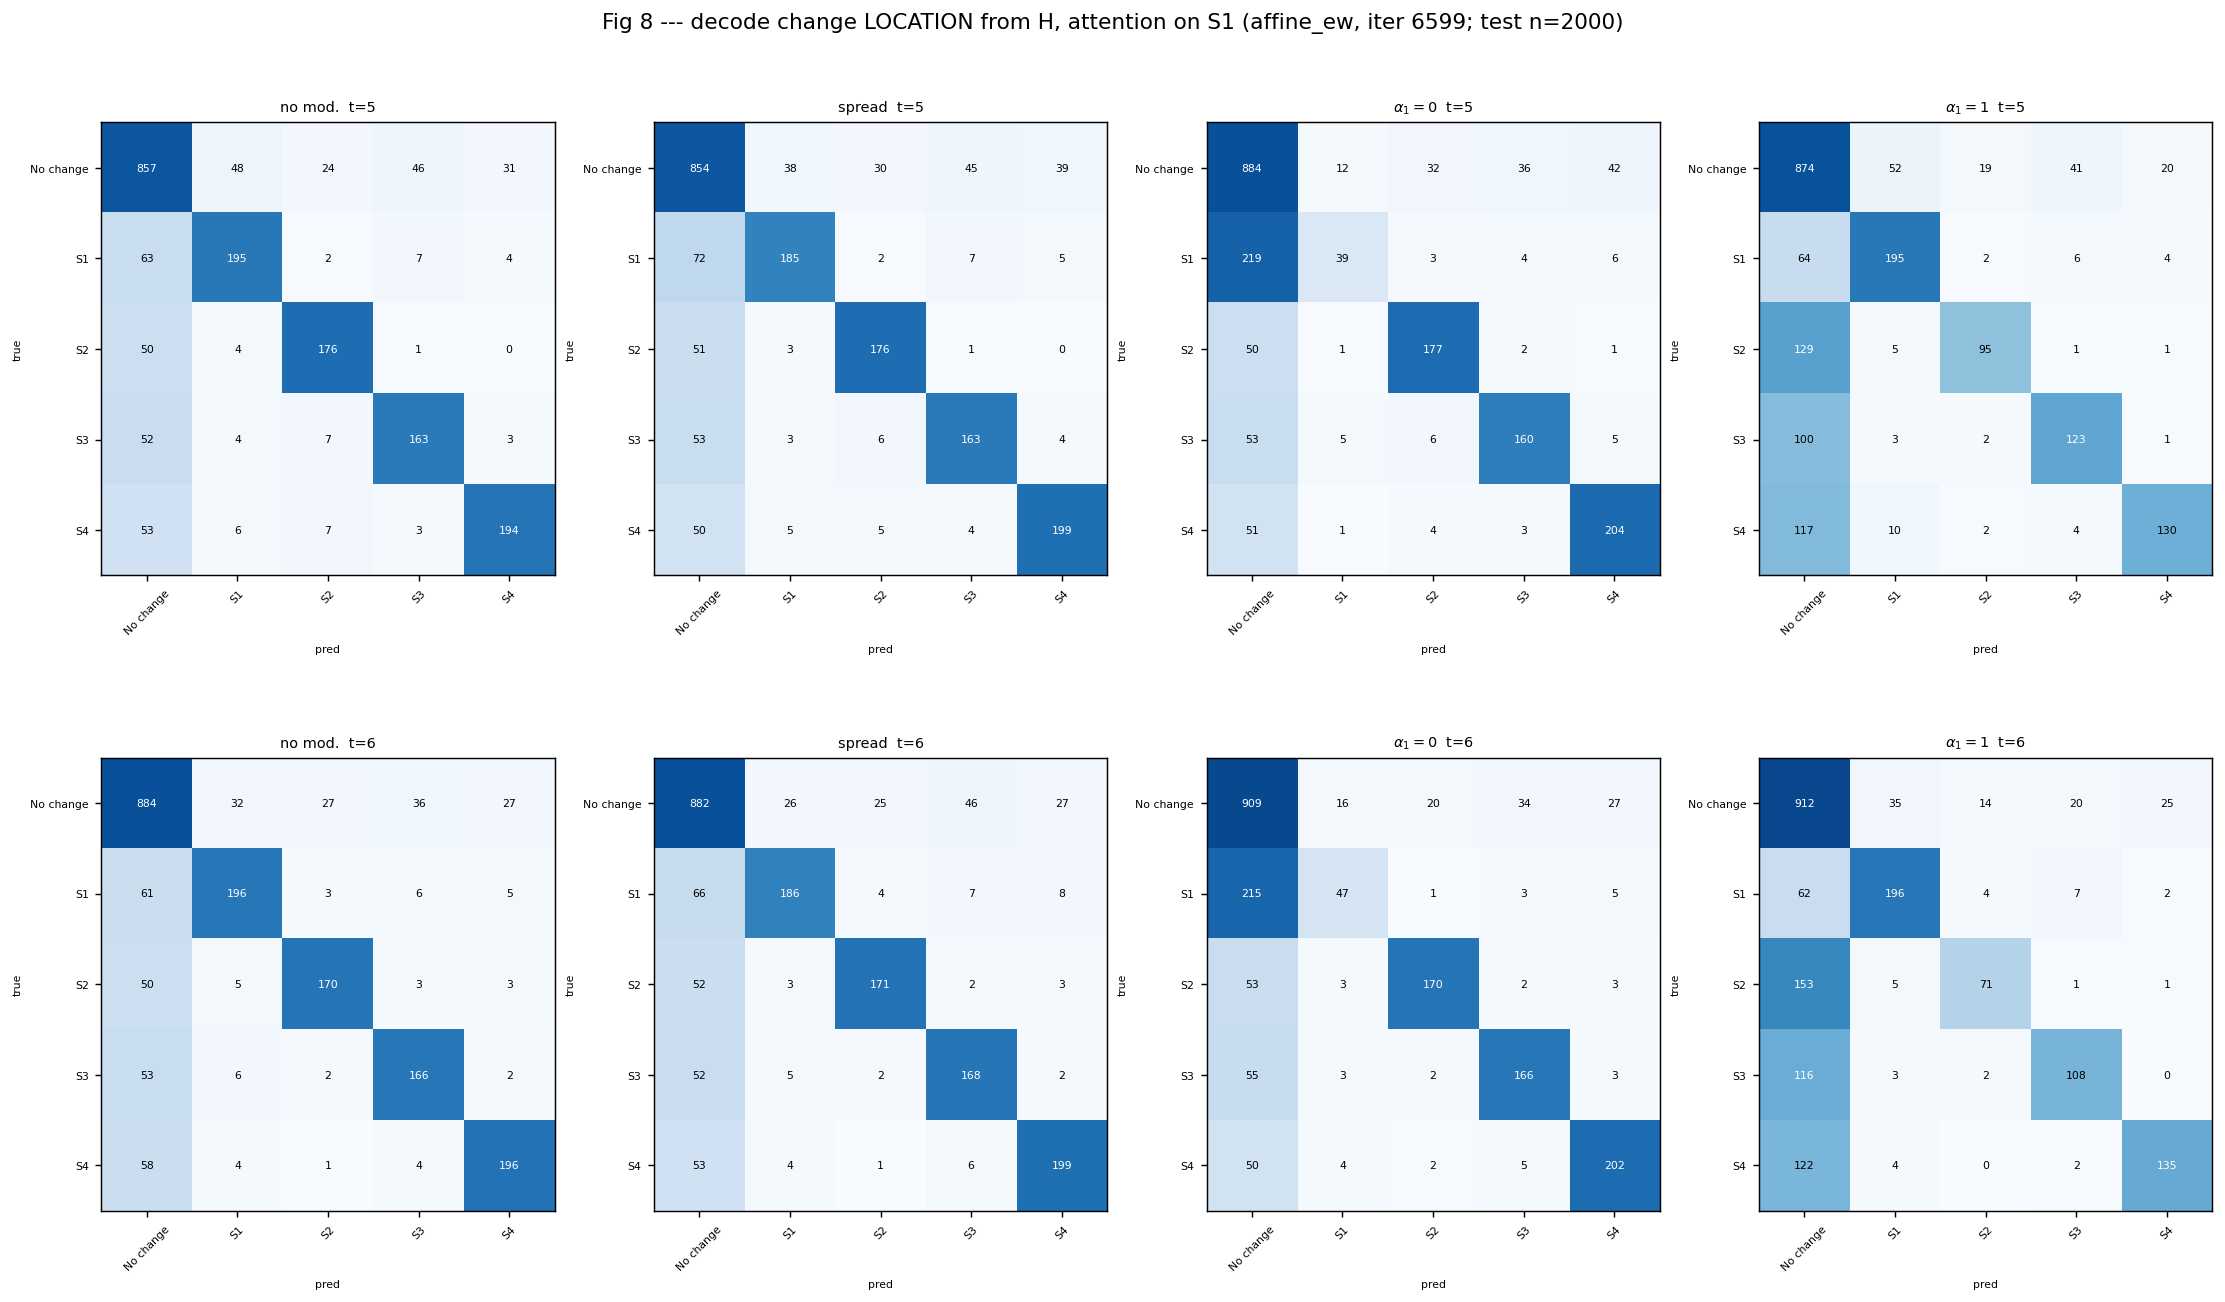
\includegraphics[width=\textwidth]{fig8_affine_ew.png}
\caption{\textbf{Fig 8 --- decode change LOCATION from $H$.} Confusion matrices (rows: $t{=}5$ top,
$t{=}6$ bottom) under \{no modulation, spread, $\alpha_1{=}0$, $\alpha_1{=}1$\}.}\label{fig:dec8}\end{figure}
\begin{figure}[h]\centering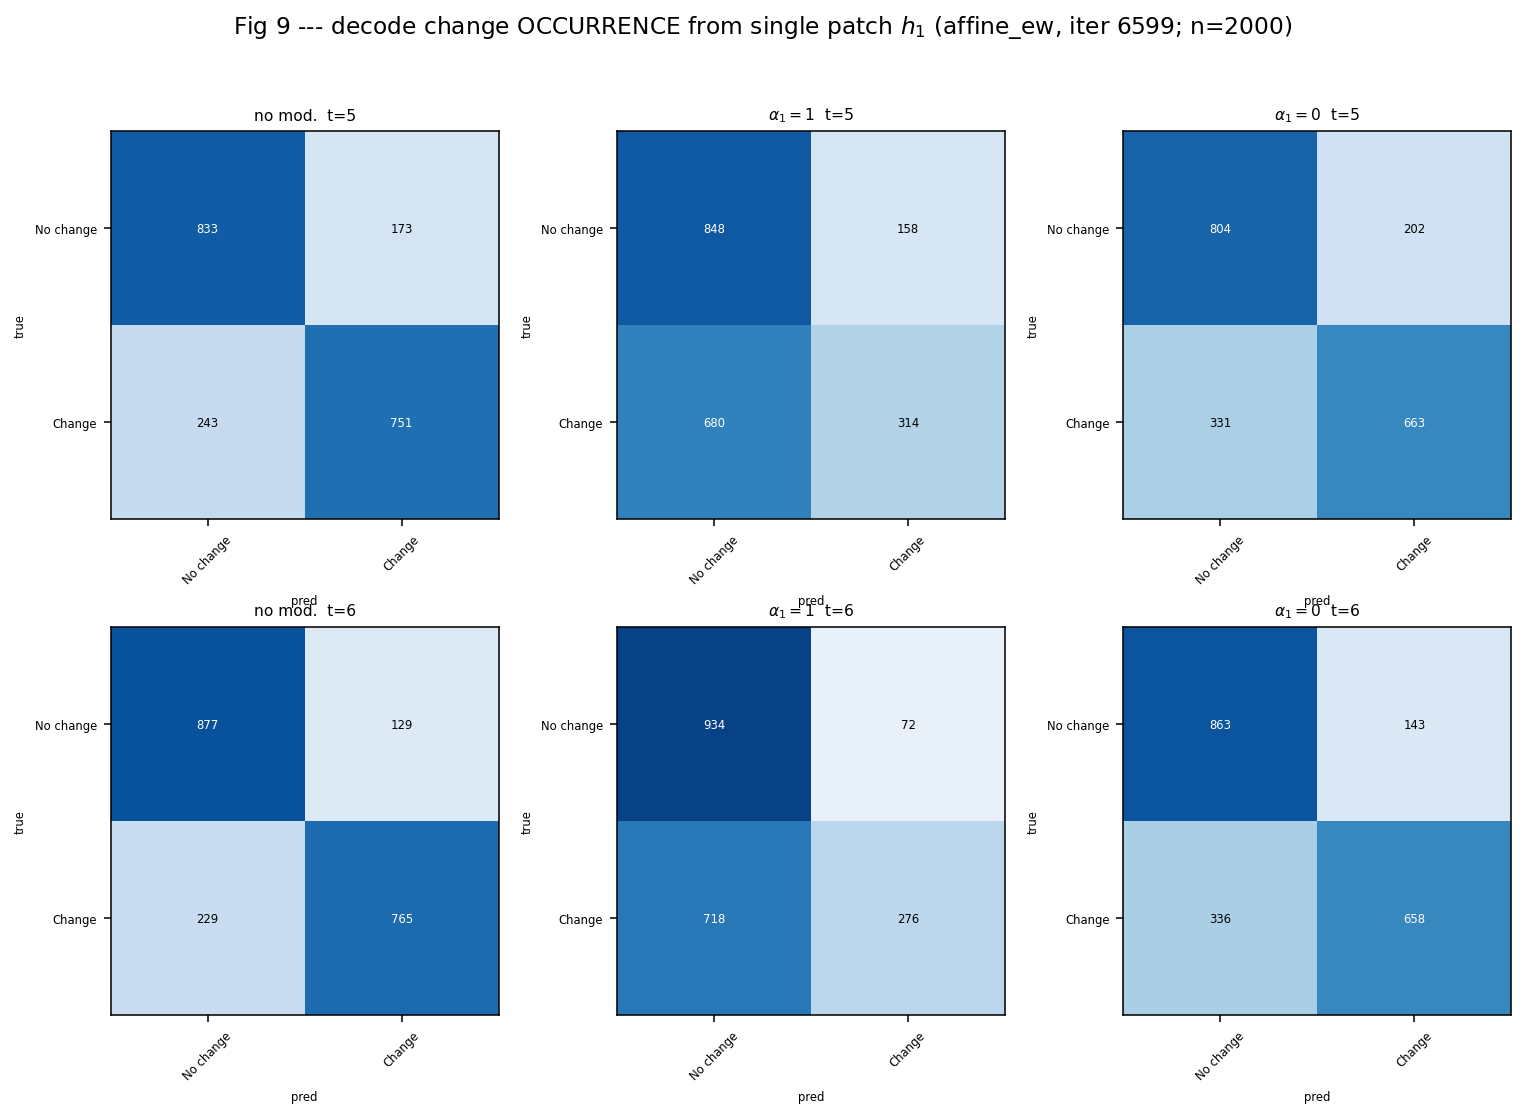
\includegraphics[width=0.85\textwidth]{fig9_affine_ew.png}
\caption{\textbf{Fig 9 --- decode change OCCURRENCE from single patch $h_1$}, $t{=}5$ (top) / $t{=}6$
(bottom), under \{no modulation, $\alpha_1{=}1$, $\alpha_1{=}0$\}.}\label{fig:dec9}\end{figure}
\begin{figure}[h]\centering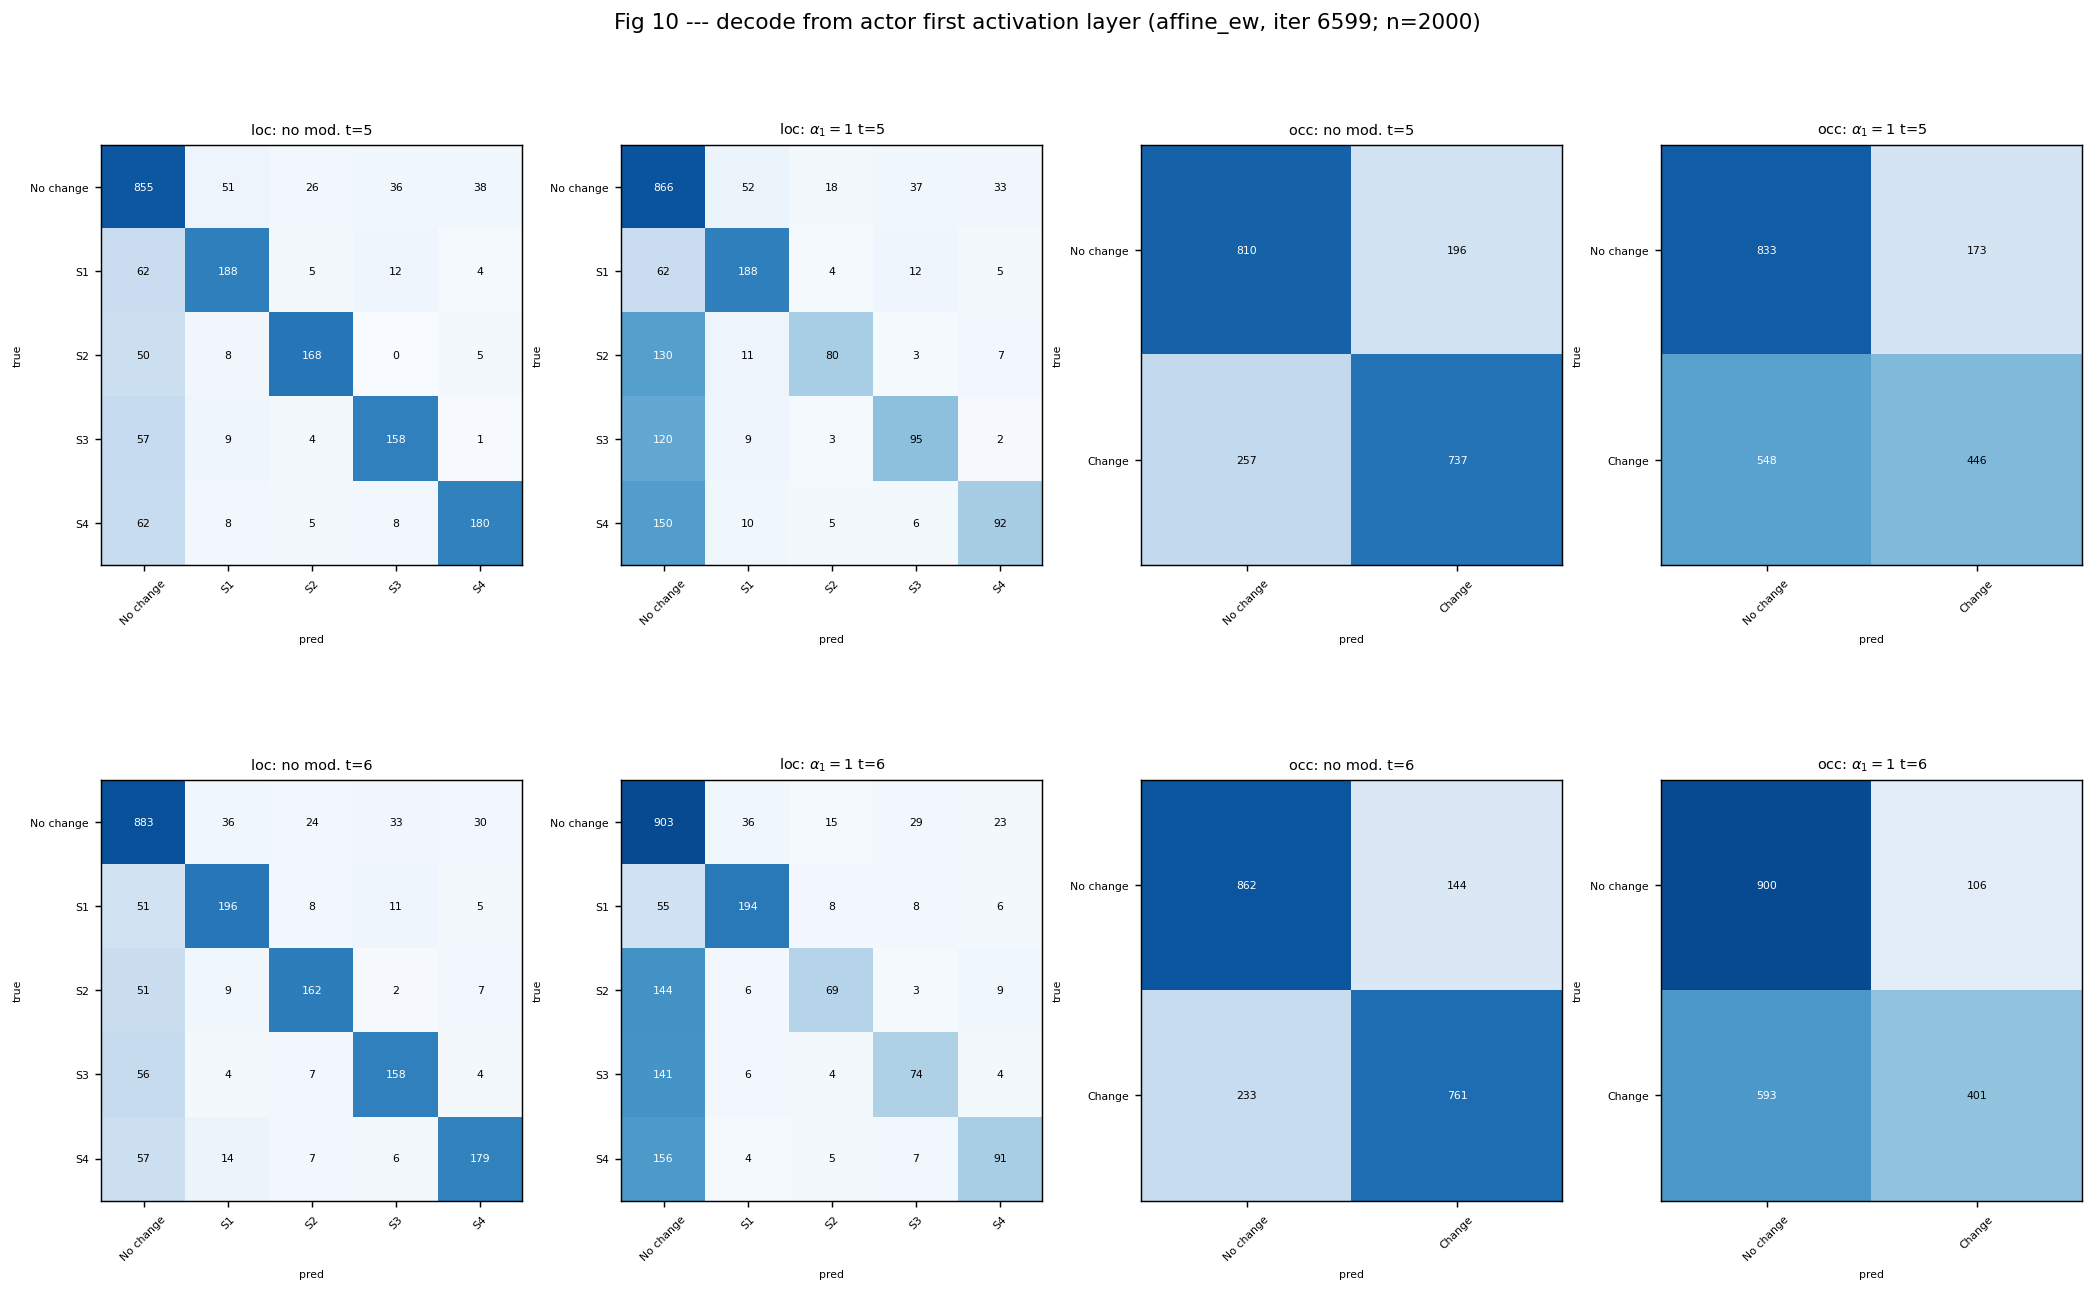
\includegraphics[width=\textwidth]{fig10_affine_ew.png}
\caption{\textbf{Fig 10 --- decode from the actor's first activation layer} (location, left; occurrence,
right), $t{=}5/6$, natural vs.\ $\alpha_1{=}1$.}\label{fig:dec10}\end{figure}
\begin{figure}[h]\centering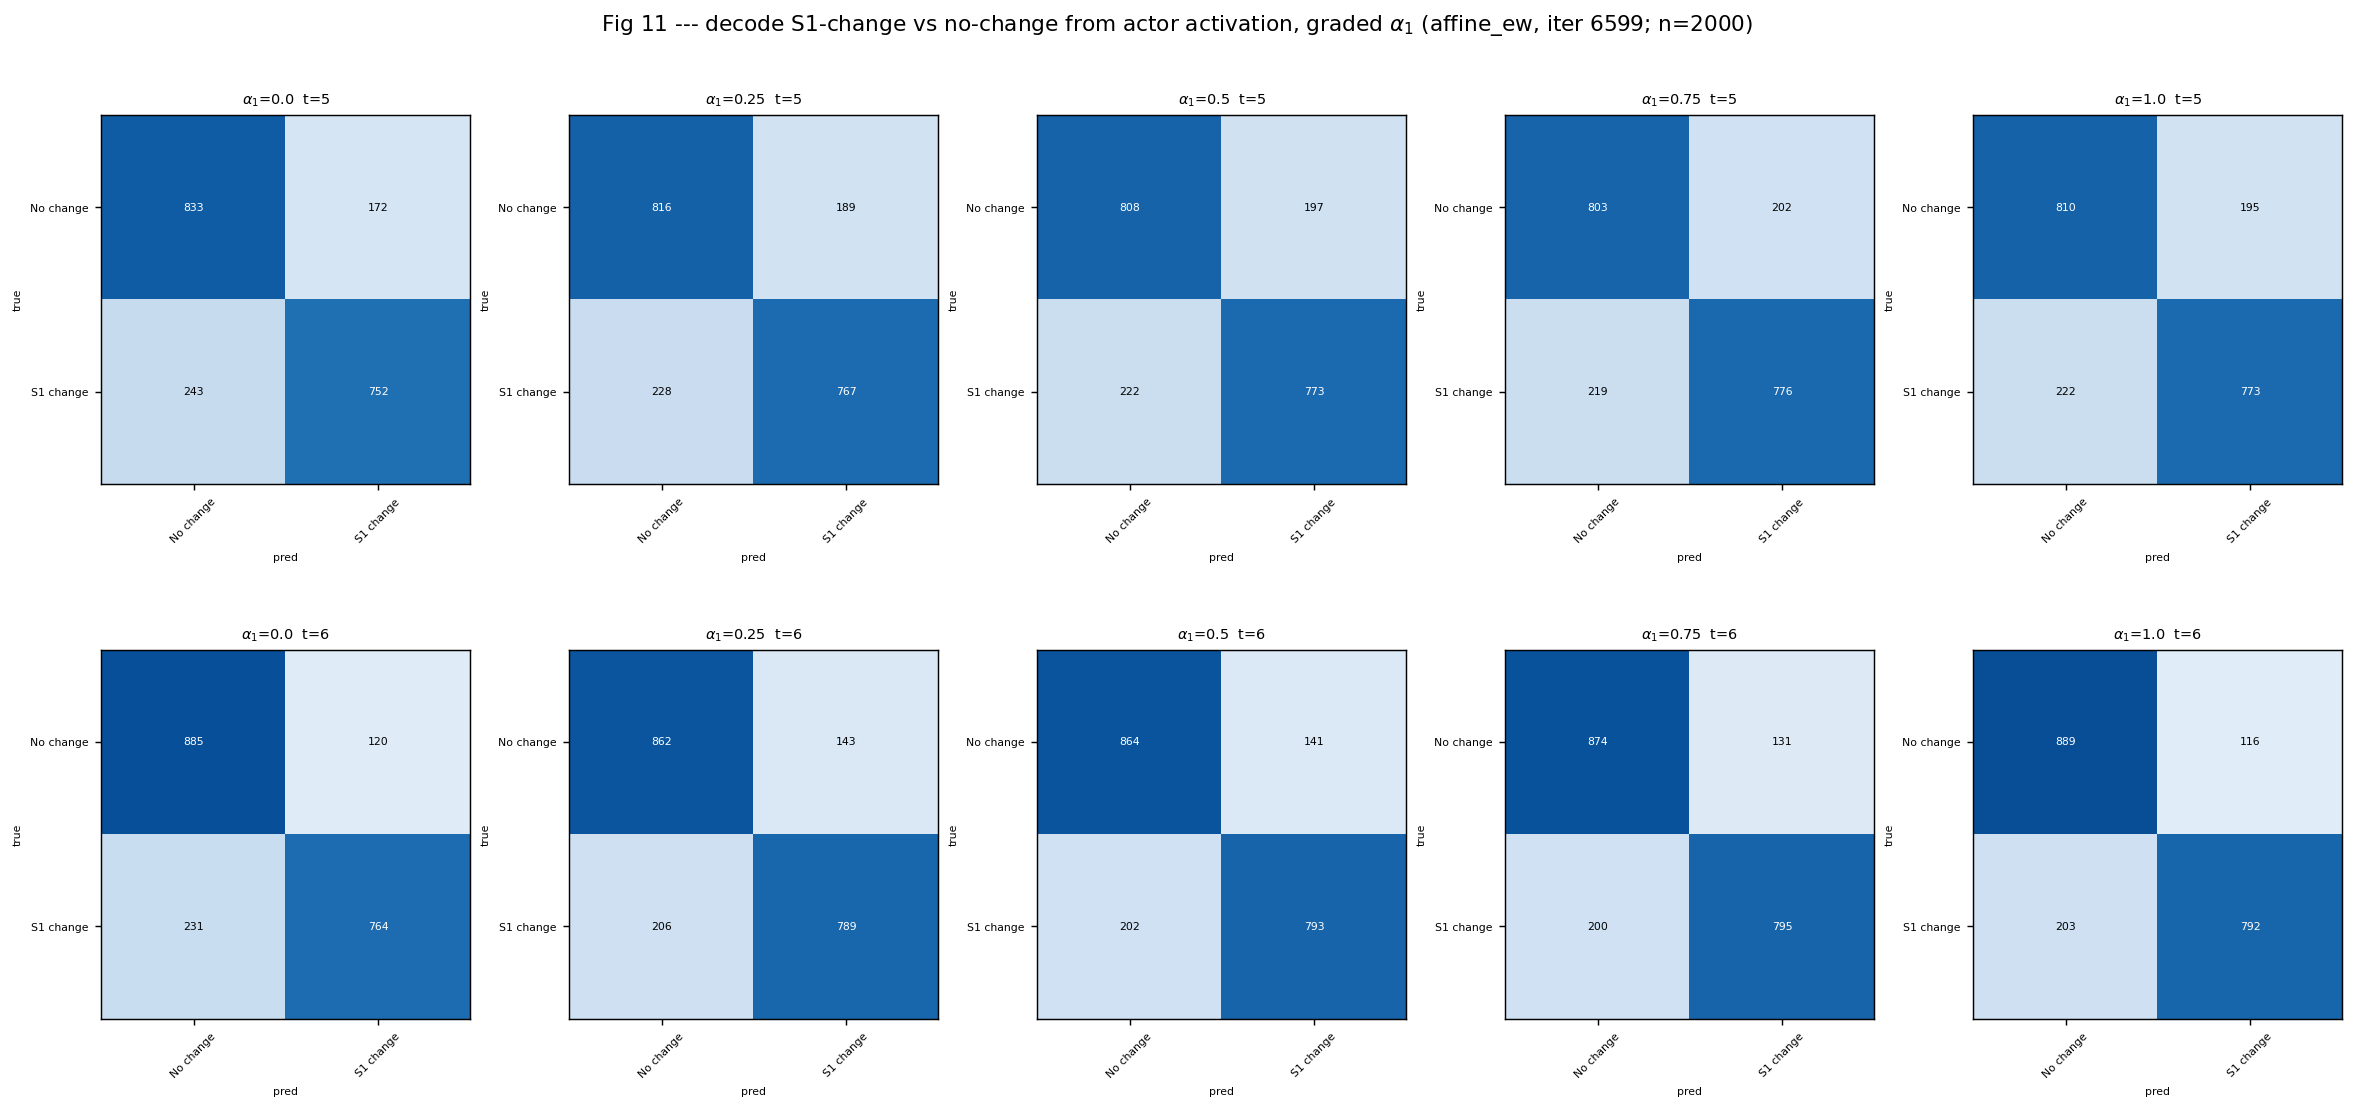
\includegraphics[width=\textwidth]{fig11_affine_ew.png}
\caption{\textbf{Fig 11 --- decode $S_1$-change vs.\ no-change from the actor activation} under graded
$\alpha_1$ inhibition ($0\to1$), $t{=}5$ (top) / $t{=}6$ (bottom).}\label{fig:dec11}\end{figure}

\section{Actor-logit geometry}
The final actor logits at the change frame lie on a competitive, anti-correlated Declare-Change vs.\
Wait axis, graded by change magnitude and largely independent of change location
(Fig.~\ref{fig:log12}). Attentional modulation shifts the distribution along this axis: enhancing
$\alpha_1$ pushes mass toward Declare-Change for $S_1$ changes, and suppressing it withdraws mass toward
Wait (Fig.~\ref{fig:log13}).

\begin{figure}[h]\centering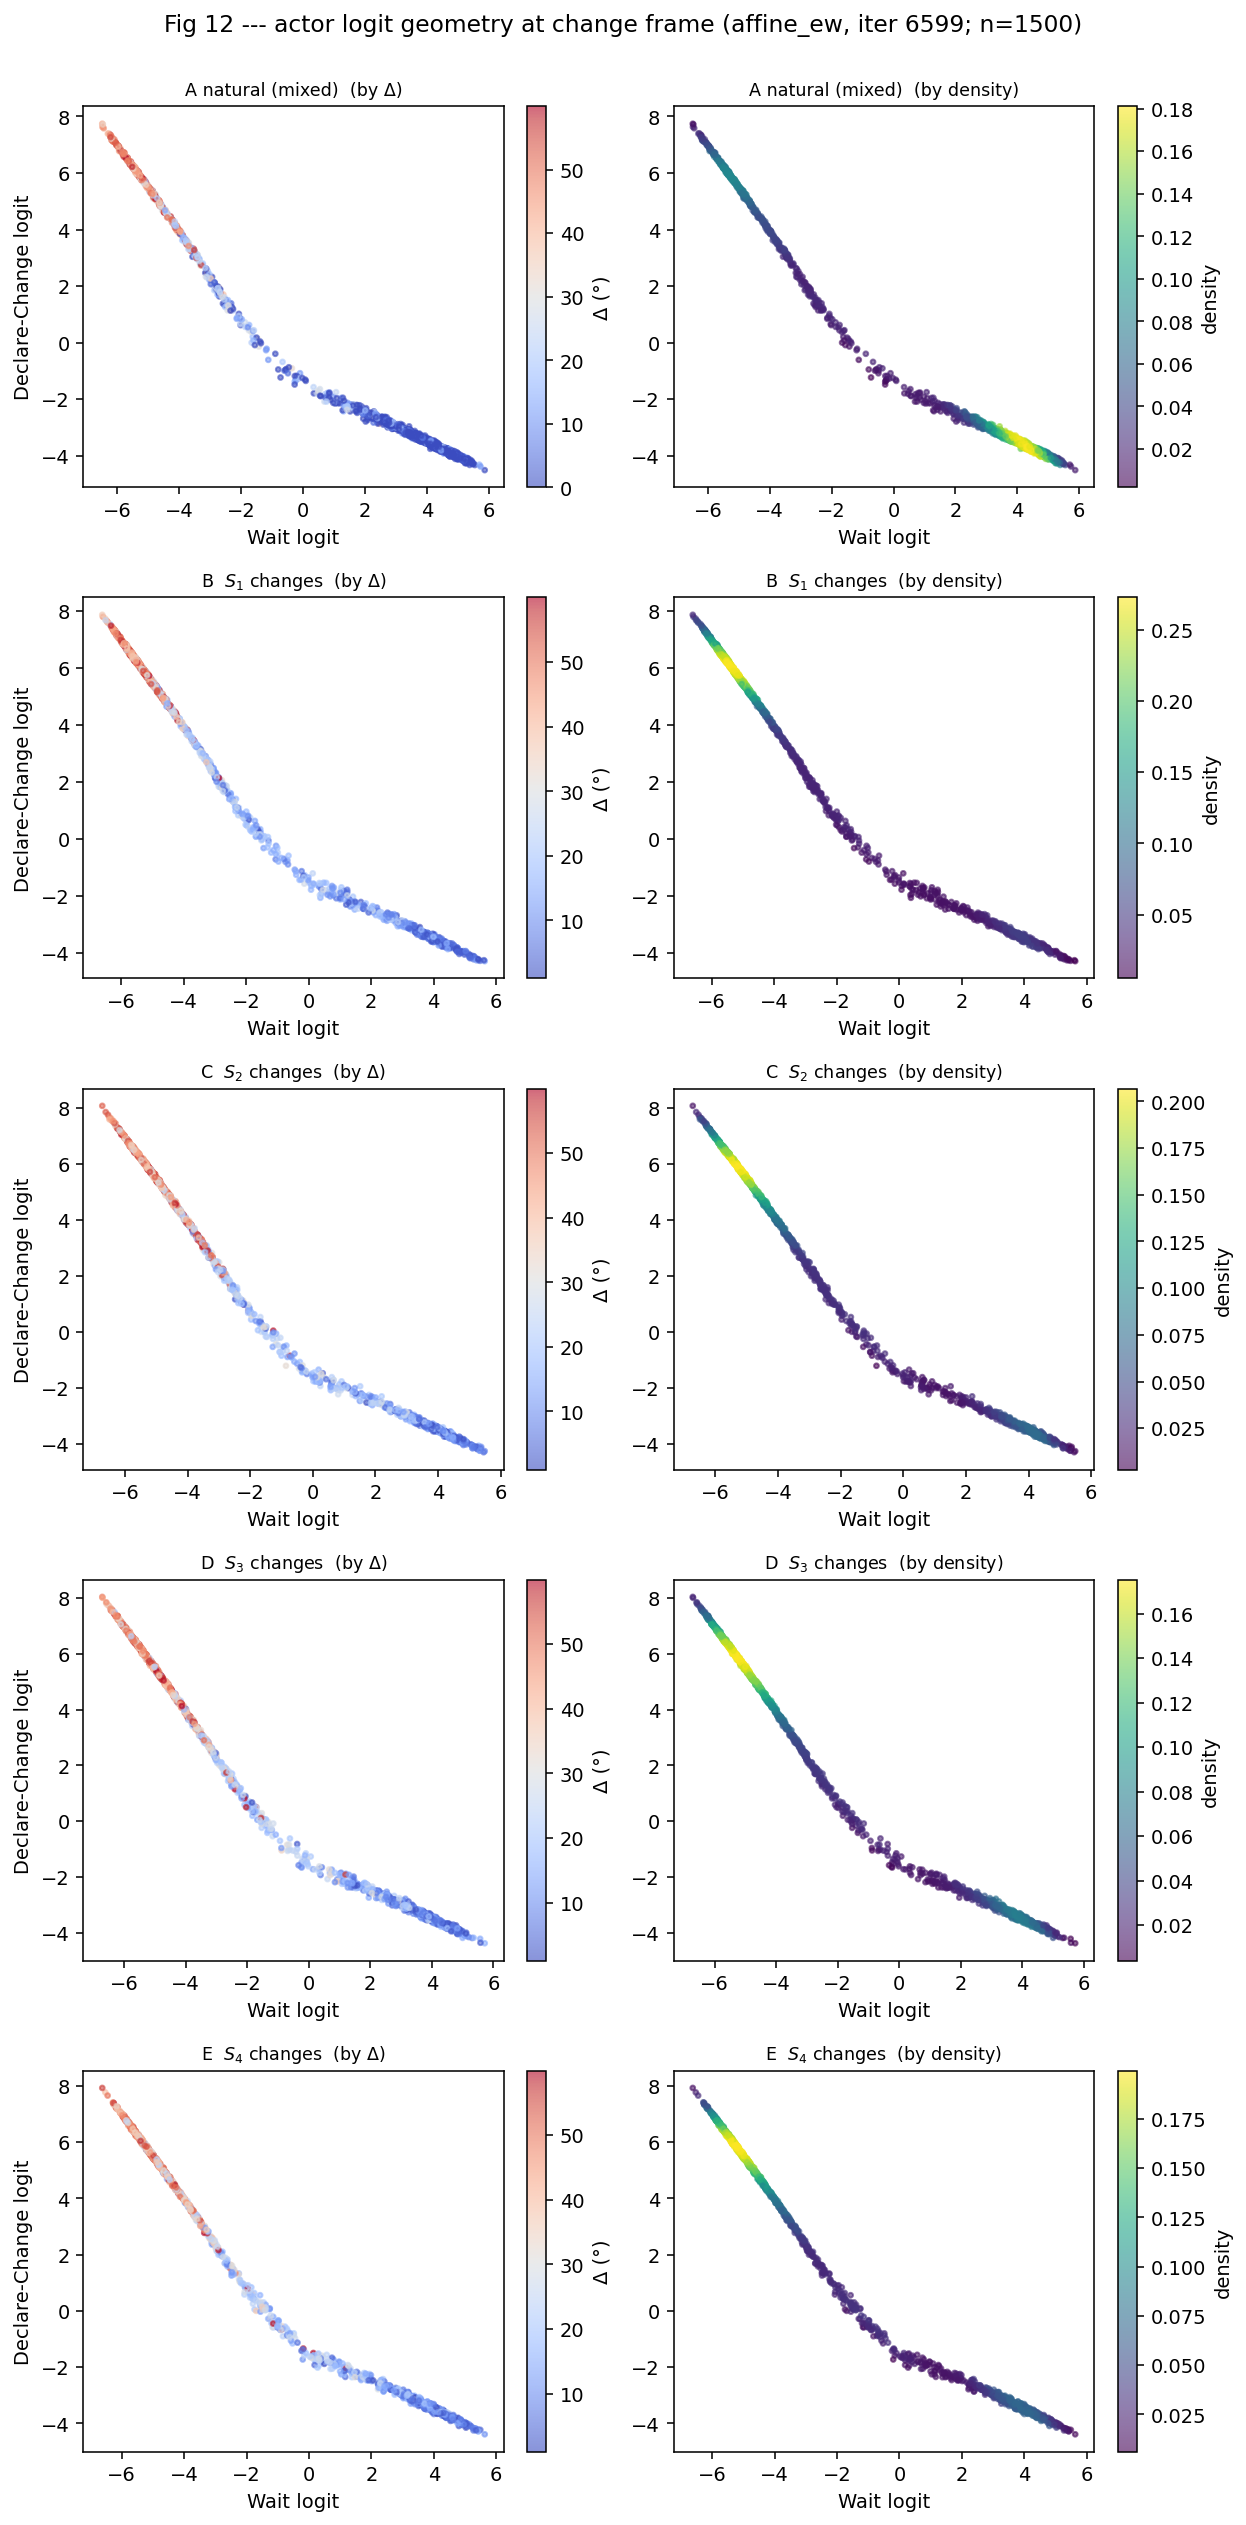
\includegraphics[width=0.62\textwidth]{fig12_affine_ew.png}
\caption{\textbf{Fig 12 --- actor logit geometry} at the change frame. A: natural mixed trials. B--E:
changes constrained to $S_1$--$S_4$. Left of each: coloured by $\Delta$; right: by 2D density.}\label{fig:log12}\end{figure}
\begin{figure}[h]\centering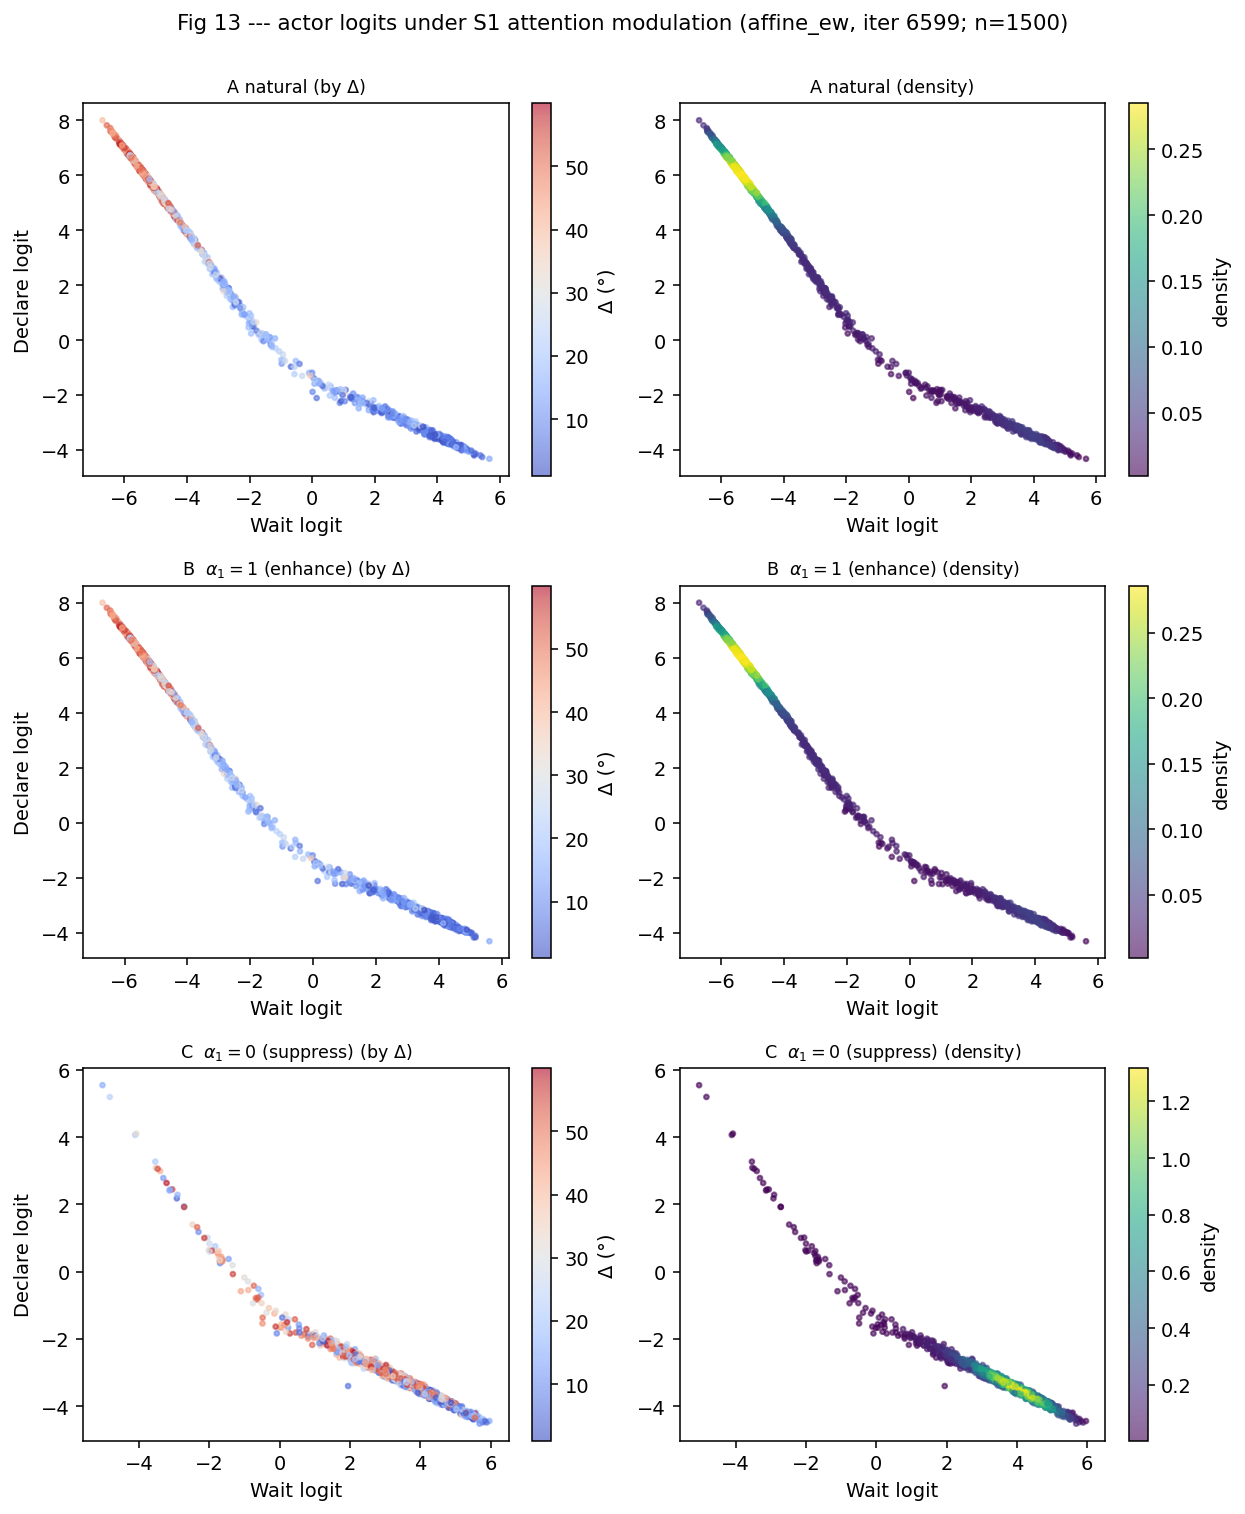
\includegraphics[width=0.62\textwidth]{fig13_affine_ew.png}
\caption{\textbf{Fig 13 --- actor logits under $S_1$ attention modulation.} A natural, B $\alpha_1{=}1$,
C $\alpha_1{=}0$; coloured by $\Delta$ (left) and density (right).}\label{fig:log13}\end{figure}

\section{Value, TD error and entropy}
From the distributional critic we read the scalar value $V(t)$; under the forced-wait rollout the
value-based TD surprise at the change, $\delta{=}\gamma V_6{-}V_5$, isolates the value jump at change
onset. The value $V$ grows monotonically with change magnitude and is higher for cued than uncued changes
(Fig.~\ref{fig:td14}B, $3.7\!\to\!4.8$), while the value-based TD surprise is positive at small $\Delta$
and declines toward zero (slightly negative) at large $\Delta$ (Fig.~\ref{fig:td14}A); graded enhancement
of attention on an uncued change modestly and non-monotonically raises the hit rate (from $52\%$ at
$\alpha_4{=}0$ to a peak $\sim\!64\%$ near $\alpha_4{=}0.5$, easing to $\sim\!60\%$ at $\alpha_4{=}1$;
a weaker, less monotone effect than the cross-attention variant) along with the TD surprise
(Fig.~\ref{fig:td14}C,D). Policy entropy is low throughout
---the greedy actor is confident---and only weakly modulated by attention; the clearer signature is the
criterion--value coupling: as attention on $S_1$ is enhanced the value rises ($V\!:4.18\to4.31$) and the
criterion falls in step ($c\!:0.31\to0.12$; Fig.~\ref{fig:ent15}).

\begin{figure}[h]\centering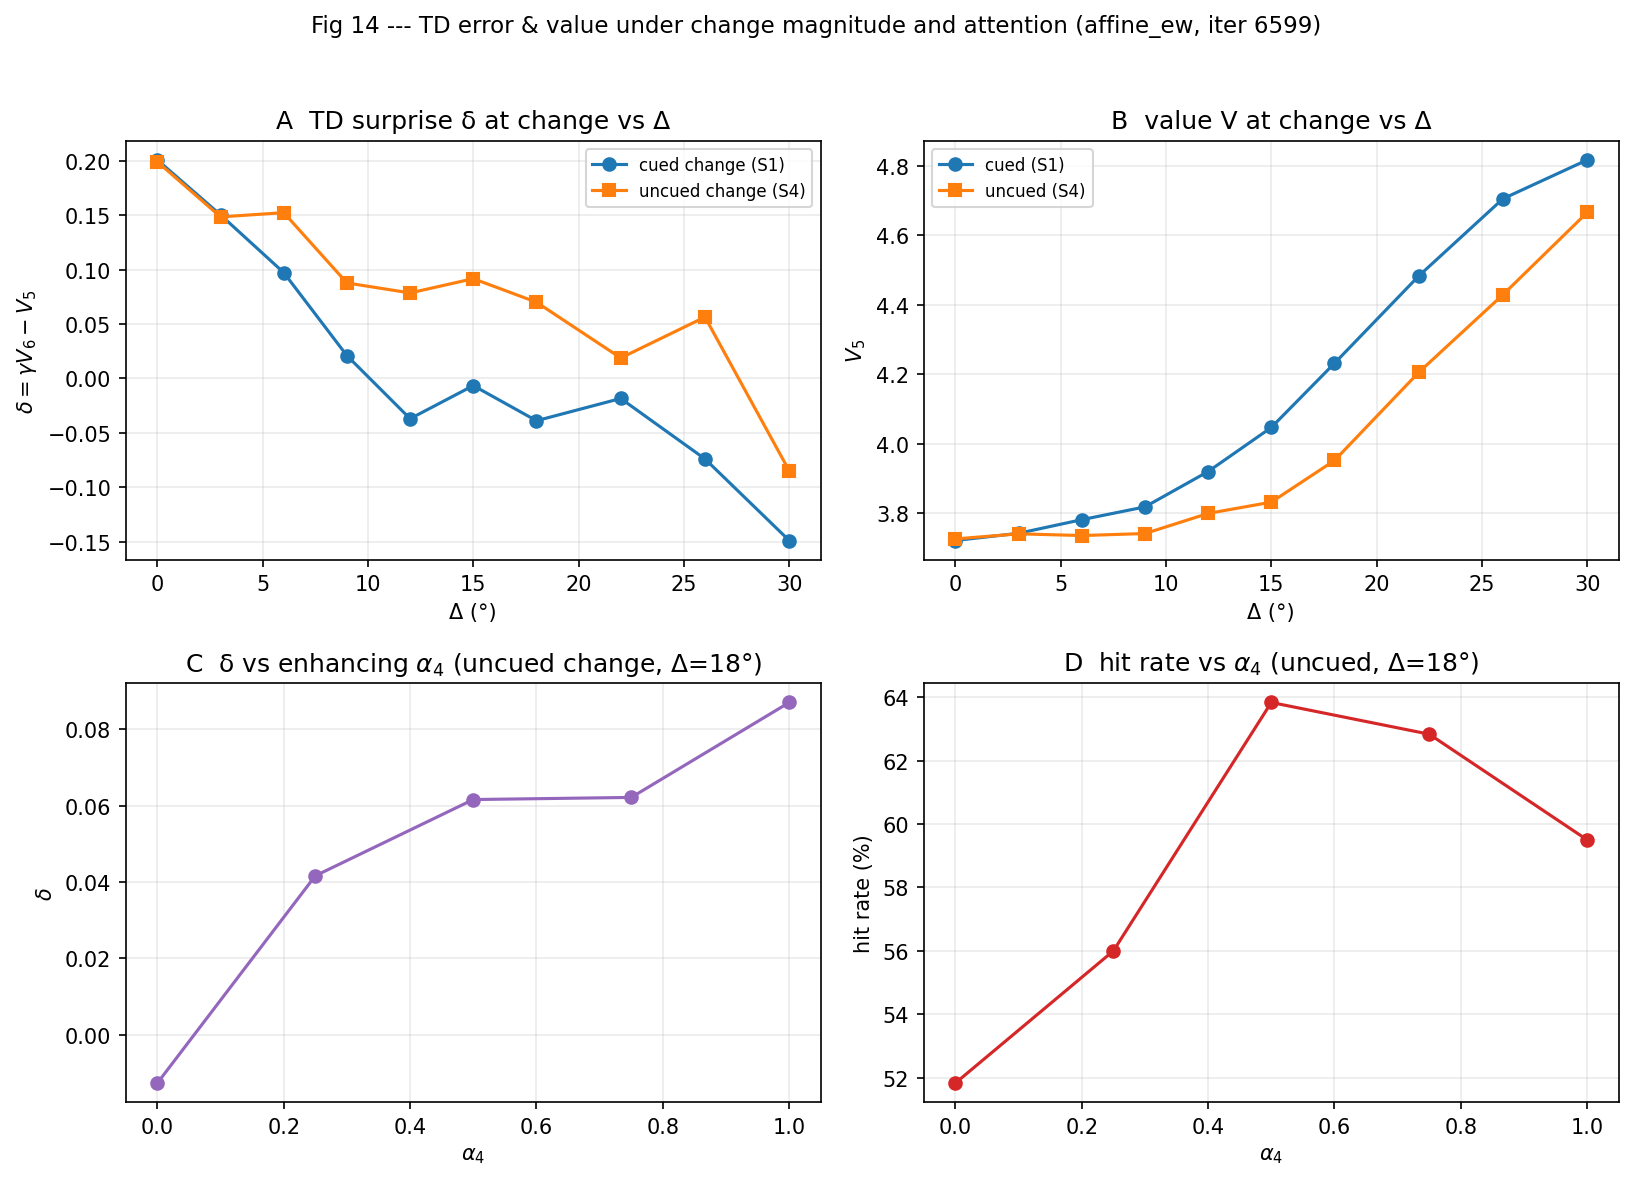
\includegraphics[width=\textwidth]{fig14_affine_ew.png}
\caption{\textbf{Fig 14 --- TD error \& value.} A: $\delta$ at change vs.\ $\Delta$, cued vs.\ uncued.
B: $V$ at change vs.\ $\Delta$. C: $\delta$ vs.\ enhancing $\alpha_4$ (uncued change). D: hit rate vs.\
$\alpha_4$.}\label{fig:td14}\end{figure}
\begin{figure}[h]\centering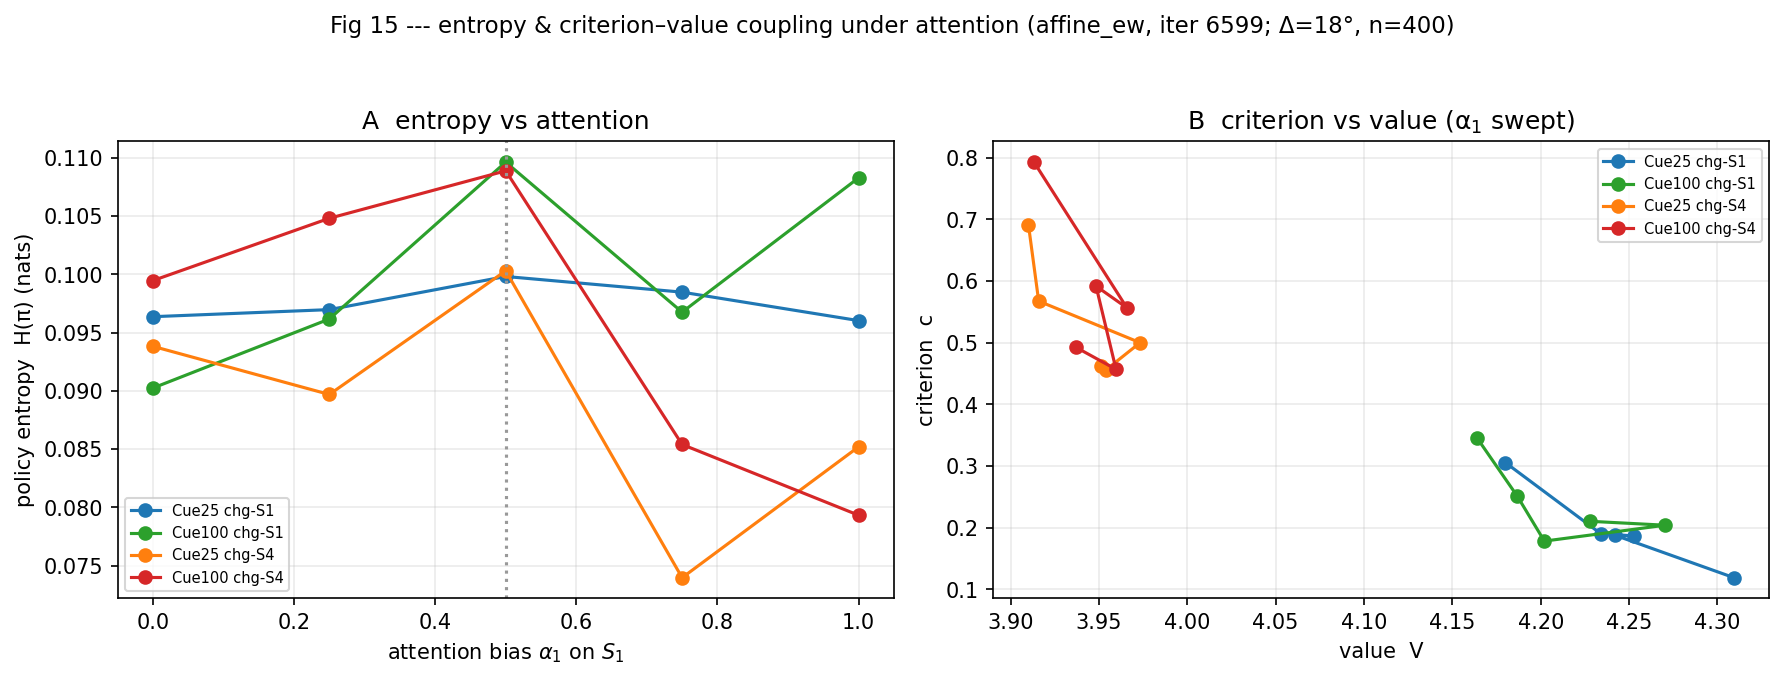
\includegraphics[width=0.95\textwidth]{fig15_affine_ew.png}
\caption{\textbf{Fig 15 --- entropy \& criterion--value coupling.} A: policy entropy at change vs.\
graded $\alpha_1$, four conditions. B: criterion $c$ vs.\ value $V$ as $\alpha_1$ is swept.}\label{fig:ent15}\end{figure}

\section{Signal detection: criterion \& sensitivity (``stimulation'' experiments)}
Treating a declared change as a ``yes'' response, we compute the signal-detection criterion
$c{=}-\tfrac12\!\big(z(\theta_H){+}z(\theta_{FA})\big)$ and sensitivity $d'{=}z(\theta_H){-}z(\theta_{FA})$
as attention on $S_1$ is biased parametrically, applied at cue-time ($t{=}1$) or change-time ($t{=}5$)
(Fig.~\ref{fig:sdt16}). Two clean signatures emerge, paralleling attentional microstimulation studies:
(i) enhancing attention on the change location lowers the \emph{criterion} (a more liberal ``change''
bias), and (ii) directing attention \emph{toward} the true change preserves/raises \emph{sensitivity}
whereas directing it \emph{away} (biasing $S_1$ when the change is at $S_4$) markedly reduces $d'$.
Notably, this graded biasing modulates the SDT decision variable even though the \emph{hard} clamps of
Fig.~\ref{fig:manip} had little behavioural effect---so for the multiplicative variant attention remains
a load-bearing decision signal in SDT terms, but only under graded (not saturating) perturbation.

\begin{figure}[h]\centering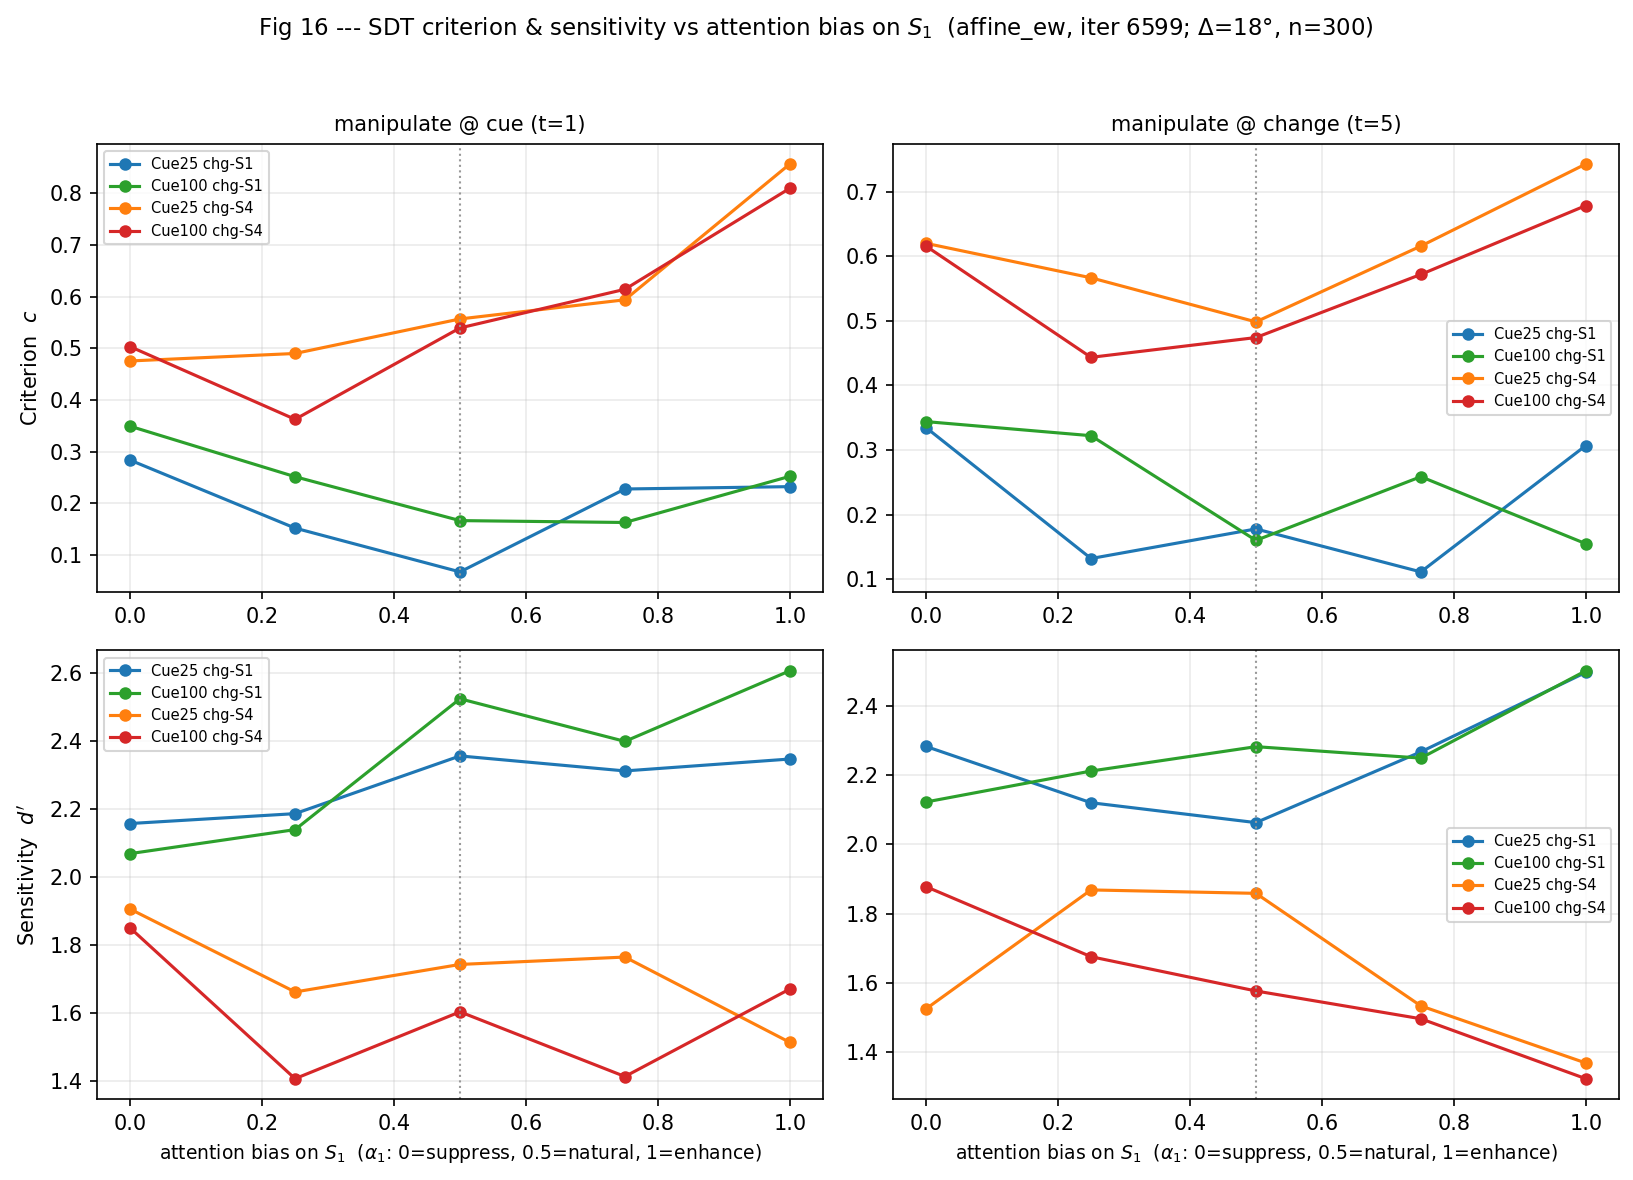
\includegraphics[width=\textwidth]{fig16_affine_ew.png}
\caption{\textbf{Fig 16 --- SDT criterion \& sensitivity vs.\ attention bias on $S_1$.} Rows: criterion
$c$, sensitivity $d'$. Columns: manipulate at cue-time ($t{=}1$) vs.\ change-time ($t{=}5$). Lines:
\{Cue $25/100\%$\}$\times$\{change at $S_1$/$S_4$\}. $\alpha_1{=}0.5$ is natural.}\label{fig:sdt16}\end{figure}

\section{Supervised vs.\ RL}
The original contrasts three training signals (supervised-actions, supervised-beliefs, RL). Our variants
are RL-only, so we faithfully reproduce the RL column across the four behavioural rows and mark the
supervised columns as out-of-scope architectural baselines that were not trained for this variant
(Fig.~\ref{fig:sup17}).

\begin{figure}[h]\centering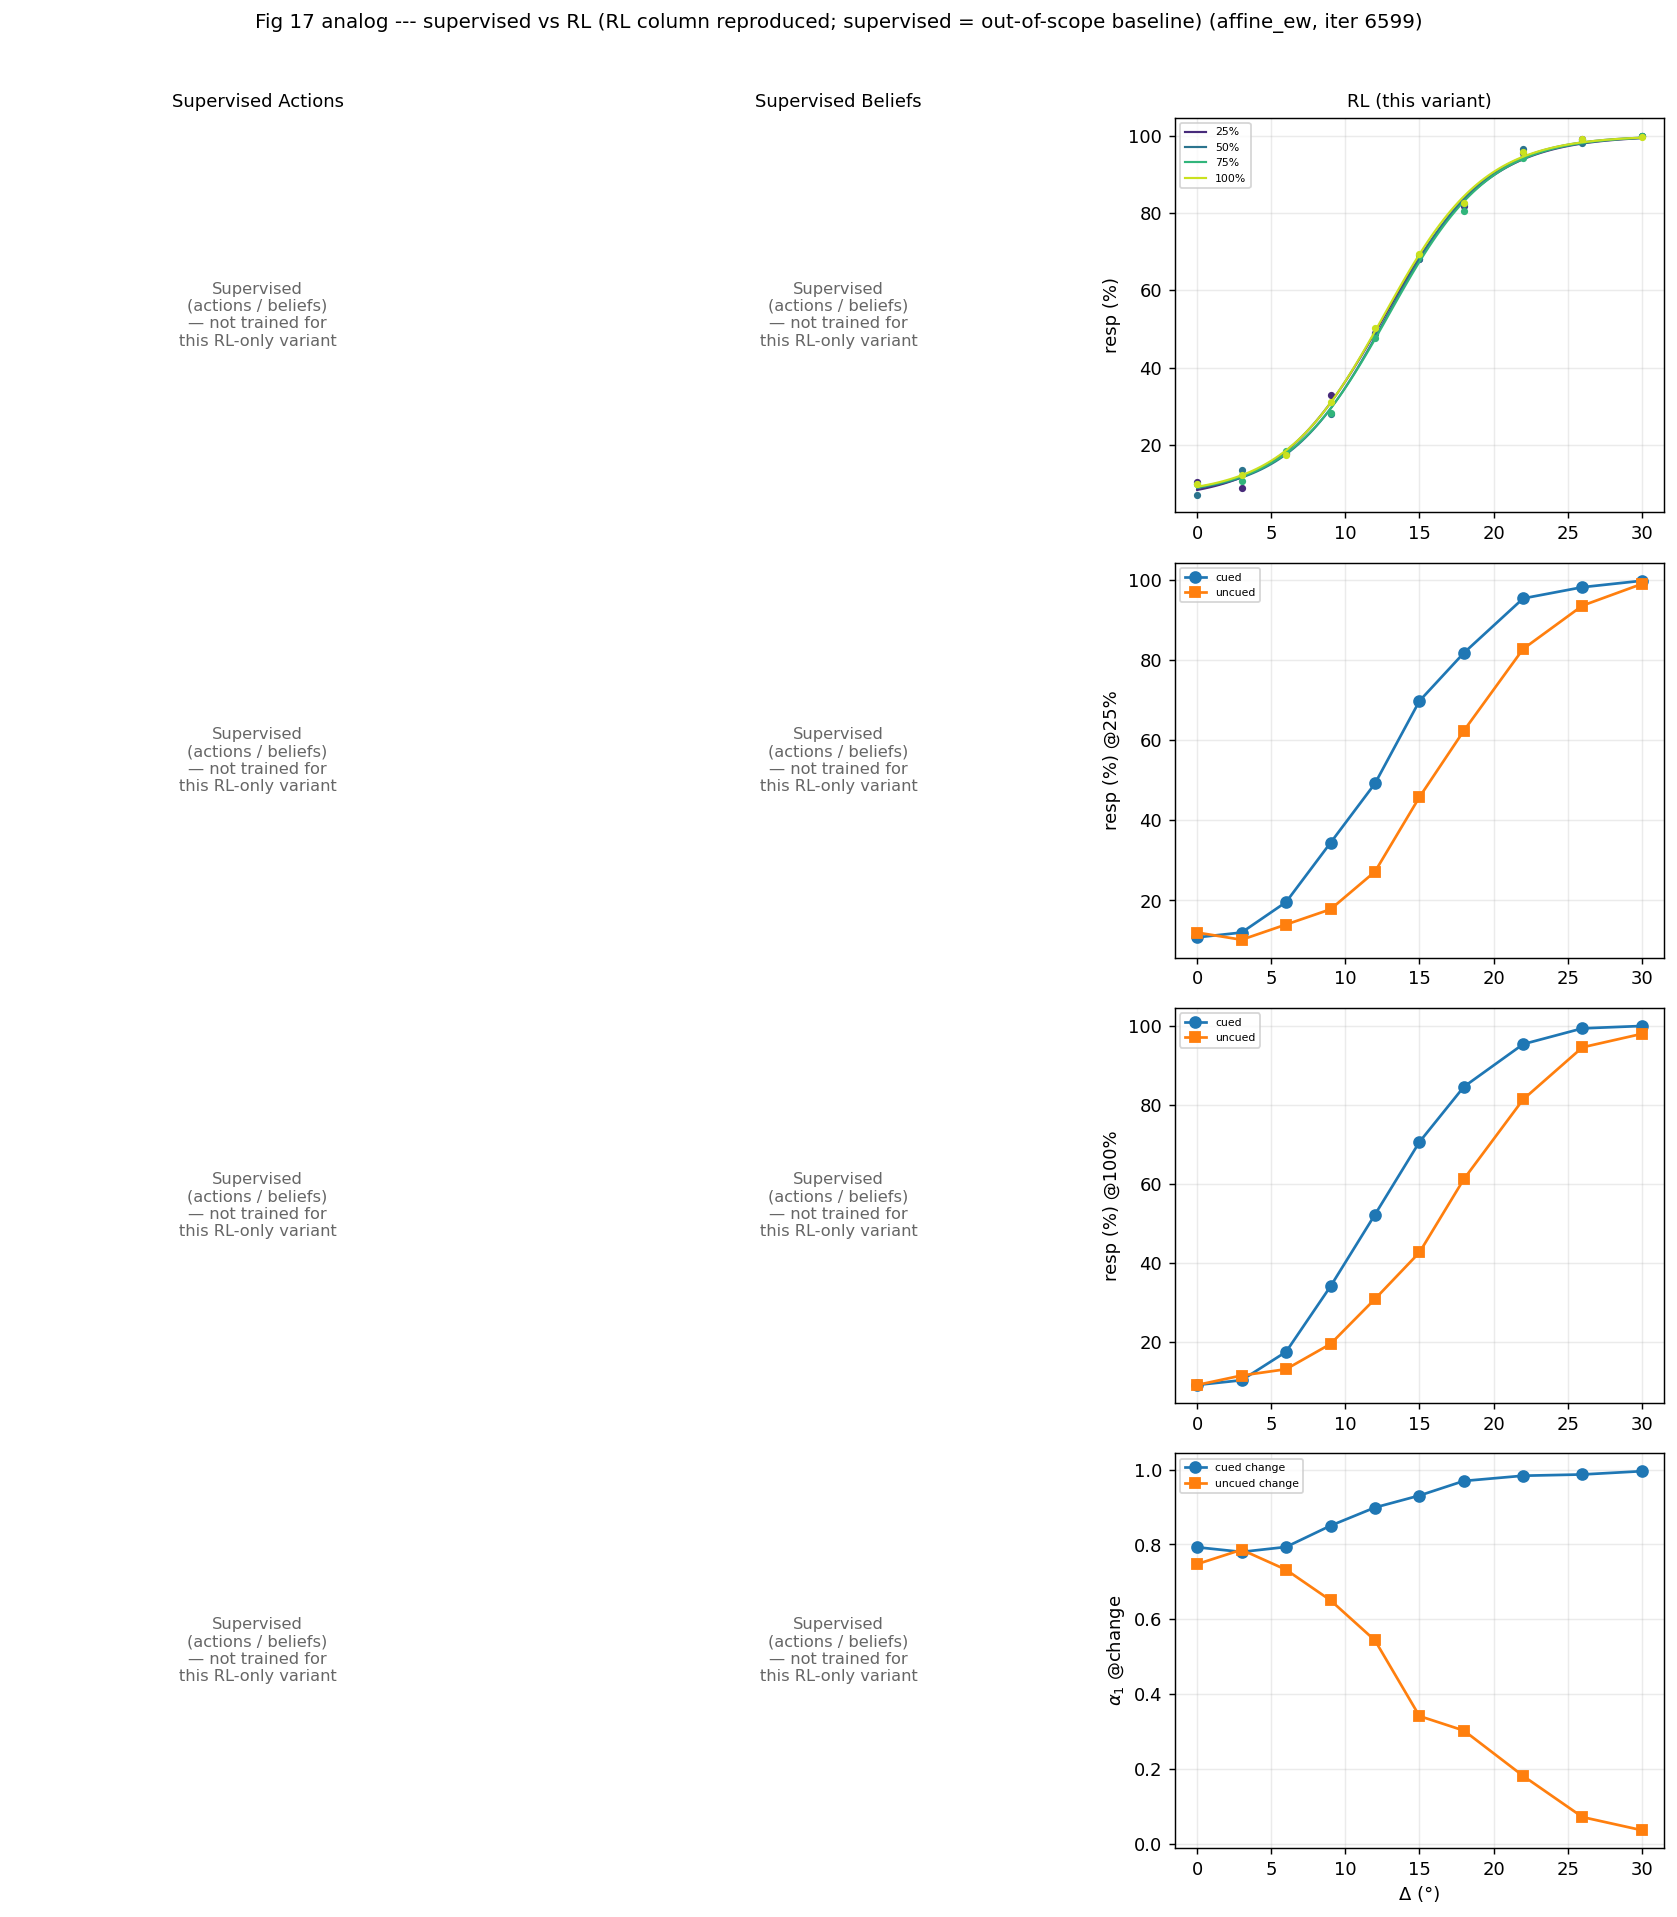
\includegraphics[width=0.9\textwidth]{fig17_affine_ew.png}
\caption{\textbf{Fig 17 analog --- supervised vs.\ RL.} RL column reproduced (response by validity;
cued vs.\ uncued at $25/100\%$; attention on $S_1$ at change vs.\ $\Delta$); supervised columns are
out-of-scope baselines for this RL-only variant.}\label{fig:sup17}\end{figure}

\section{Discussion}
The compact, pixel-trained multiplicative-gating variant reproduces the \emph{shape} of primate-like
signatures across the whole figure set: sigmoidal psychometrics/chronometrics, a cued$>$uncued spatial
benefit, anticipatory maintenance of spatial priority, self-attention amplification of the change signal
across memory slots, a competitive actor-logit decision axis, a distributional value jump at the change,
and the graded SDT criterion/sensitivity signatures of attentional ``stimulation.'' It \emph{diverges}
from the original---and from the companion cross-attention variant---in two ways. First, as for the
cross-attention variant, it is \emph{invariant to displayed cue validity}: it reads the validity ring at
the cue frame but does not maintain it, so the validity-graded modulation of the original
($d_{\mathrm{mem}}{=}1024$, VAE) does not emerge. Second, its attention is a \emph{weaker hard causal
lever}: saturating clamps ($\alpha{=}0/1$) barely move behaviour and produce no ``dual effect,'' whereas
graded biasing still modulates the SDT decision variable. This is consistent with the multiplicative
gate entering as a soft rescaling rather than a competitive key/value, and it dissociates two senses of
``causal attention''---graded decision influence, preserved; hard override, weak.

\section{Methods (variant)}
\textbf{Front-end.} Each $25\times25\times3$ patch is encoded by a shared SE-ResNet to
$\hat o_i\in\mathbb R^{128}$; the token is $[\hat o_i\Vert\rho_i\Vert\tau]\in\mathbb R^{140}$.
\textbf{Multiplicative gating.} The memory produces an element-wise affine transform of the visual
tokens, $X'{=}\gamma(H^{(t-1)})\odot X+\beta(H^{(t-1)})$, which then self-attend ($Q,K,V$ from $X'$,
$A=\mathrm{softmax}(QK^\top/\sqrt{140})$ over the four tokens, $Z=X'+AV$). \textbf{Memory.} A per-patch spatial
xLSTM, $d_{\mathrm{mem}}{=}128$; the flattened cell $H$ is read out. \textbf{Training.} Distributional
actor--critic on sparse reward with an auxiliary V-JEPA temporal self-distillation loss (4 heads
$\times$ 256 prototypes). \textbf{Analyses.} Behaviour uses $n{=}300$ trials/point; psychometrics fit a
4-parameter logistic $P(\Delta)=A+(1{-}A{-}B)/(1+e^{-(\Delta-D)/C})$. Attention is causally manipulated
by additively biasing the pre-softmax key scores of a location. Decoders are trained on natural states
and evaluated under modulation. SDT quantities use hit rate on change trials and false-alarm rate on
no-change trials at $\Delta{=}18^\circ$.

\end{document}
